\documentclass[10.5pt,a4paper]{article}

\usepackage[utf8]{inputenc}
\usepackage[T1]{fontenc}
\usepackage{lmodern}
\usepackage[margin=0.72in,top=0.7in,bottom=0.7in]{geometry}
\usepackage{amsmath,amssymb,amsfonts}
\usepackage{graphicx}
\usepackage{booktabs,tabularx,array}
\usepackage{xcolor}
\usepackage{fancyhdr}
\usepackage{titlesec}
\usepackage{microtype}
\usepackage{enumitem}
\usepackage{subcaption}
\usepackage[most]{tcolorbox}
\usepackage[colorlinks=true,linkcolor=navyblue,citecolor=tealblue,urlcolor=navyblue]{hyperref}

% --- Color Palette ---
\definecolor{navyblue}{RGB}{20, 45, 110}
\definecolor{tealblue}{RGB}{13, 148, 136}
\definecolor{darkslate}{RGB}{30, 41, 59}
\definecolor{lightbg}{RGB}{248, 250, 252}
\definecolor{cardborder}{RGB}{226, 232, 240}
\definecolor{accentgreen}{RGB}{16, 185, 129}
\definecolor{accentamber}{RGB}{217, 119, 6}

% --- Headers & Footers ---
\pagestyle{fancy}
\fancyhf{}
\fancyhead[L]{\small\sffamily\color{gray} MagMat $\cdot$ Physics-Grounded Screening \& Discovery Guide}
\fancyhead[R]{\small\sffamily\color{gray} Sachin Poudel}
\fancyfoot[C]{\small\sffamily\color{darkslate}\thepage}
\renewcommand{\headrulewidth}{0.4pt}

% --- Section Styling ---
\titleformat{\section}{\Large\sffamily\bfseries\color{navyblue}}{\thesection}{0.5em}{}[\titlerule]
\titleformat{\subsection}{\large\sffamily\bfseries\color{darkslate}}{\thesubsection}{0.4em}{}
\titleformat{\subsubsection}{\normalsize\sffamily\bfseries\color{tealblue}}{\thesubsubsection}{0.3em}{}

\titlespacing*{\section}{0pt}{9pt}{4pt}
\titlespacing*{\subsection}{0pt}{7pt}{3pt}
\titlespacing*{\subsubsection}{0pt}{5pt}{2pt}

\setlist{itemsep=1.5pt, topsep=2pt, parsep=0pt}
\setlength{\parskip}{3pt}
\setlength{\parindent}{0pt}

\tcbset{
  enhanced,
  boxrule=0.9pt,
  arc=2.5mm,
  fonttitle=\sffamily\bfseries,
  colback=lightbg,
  colframe=cardborder,
  boxsep=3pt,
  left=7pt, right=7pt, top=5pt, bottom=5pt
}

\newtcolorbox{infobox}[2][]{
  colframe=navyblue,
  colback=navyblue!3!white,
  coltitle=white,
  title=#2,
  fonttitle=\sffamily\bfseries\small,
  #1
}

\newtcolorbox{takeawaybox}[1][Key Takeaway]{
  colframe=tealblue,
  colback=tealblue!4!white,
  coltitle=white,
  title=#1,
  fonttitle=\sffamily\bfseries\small
}

\begin{document}

% --- Title Block ---
\begin{center}
  {\LARGE\sffamily\bfseries\color{navyblue} MagMat: Physics-Grounded Screening \& Discovery}\\[0.3em]
  {\large\sffamily\color{darkslate} Architecture and Methodology Guide for Sustainable Permanent Magnets}\\[0.4em]
  {\normalsize\sffamily\bfseries Sachin Poudel}\\[0.2em]
  {\small\sffamily\color{gray} Open-Source Platform Guide}
\end{center}
\vspace{0.4em}

\begin{infobox}{Executive Summary}
\small
Permanent magnets power electric vehicle traction motors and direct-drive wind generators. Today's highest-performance magnets depend heavily on critical rare-earth elements (Nd, Dy, Tb), whose mining and processing carry severe supply risks and environmental costs.

This framework establishes a physics-grounded screening and discovery methodology for sustainable, rare-earth-free permanent magnets. It unites three complementary capabilities:
\begin{enumerate}[leftmargin=*]
  \item \textbf{Analytical Condensed-Matter Ceilings:} Four classical physical laws (Slater-Pauling, Stoner exchange, Kronmüller micromagnetics, and Maxwell limits) providing parameter-free theoretical upper bounds.
  \item \textbf{Trained Machine Learning Pipeline:} Multi-task regression and classification ensembles predicting realistic experimental properties ($T_C$, $T_N$, ground-state phase, $M_s$, $H_c$, $K_1$, $(BH)_{\max}$) accompanied by non-parametric conformal uncertainty intervals.
  \item \textbf{3D Atomistic Foundation AI:} Crystal diffusion (DAO) and equivariant message passing (MACE) resolving polymorph degeneracy and addressing the 89\% microstructural defect gap.
\end{enumerate}
\end{infobox}

% =========================================================================
\section{Methodological Architecture}
% =========================================================================

\begin{figure}[htbp]
  \centering
  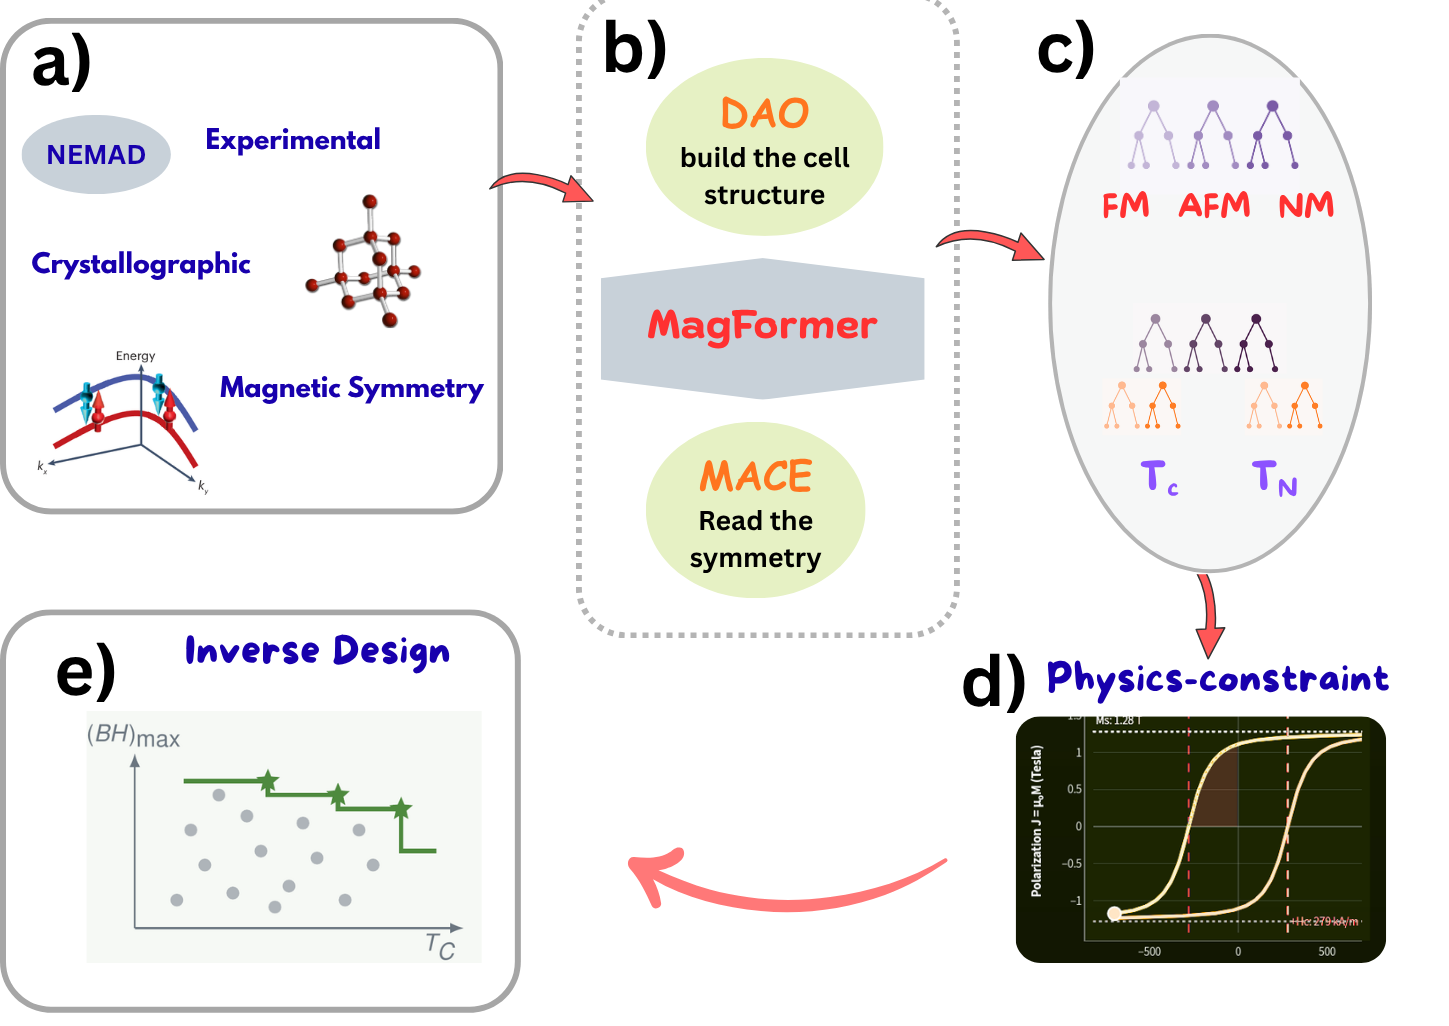
\includegraphics[width=0.88\textwidth]{figures/methodology.png}
  \vspace{-0.3em}
  \caption{\textbf{Multi-Scale Integrated Architecture.} (a) Experimental datasets from NEMAD and literature with crystallographic and magnetic symmetry. (b) 3D foundation AI: DAO crystal diffusion (cell structure and $E_{\text{hull}}$ stability), MagFormer compositional transformer, and MACE equivariant symmetry. (c) Trained machine learning models: multi-model classifier for ground-state phase (FM, AFM, NM) and dynamic regression ensembles for transition temperatures ($T_C, T_N$). (d) Physics-constraint benchmarking against analytical condensed-matter ceilings (Kronmüller micromagnetics, Slater-Pauling, Maxwell bound). (e) Multi-objective inverse Pareto discovery ($(BH)_{\max}$ vs $T_C$).}
  \label{fig:workflow}
\end{figure}

The architecture ensures that every composition proposed by machine learning is strictly benchmarked against physical bounds before experimental synthesis or intensive DFT simulations.

% =========================================================================
\section{The Four Analytical Condensed-Matter Ceilings}
% =========================================================================

We implement four classical physical rules that turn chemical stoichiometry into hard performance ceilings without parameter fitting:

\begin{table}[htbp]
\centering
\small
\renewcommand{\arraystretch}{1.15}
\begin{tabularx}{\textwidth}{lp{3.6cm}X}
\toprule
\textbf{\#} & \textbf{Physical Bound} & \textbf{Core Question Answered \& Governing Physics} \\
\midrule
\textbf{1} & \textbf{Slater-Pauling Atomic Ceiling} & \emph{What is the absolute maximum magnetization?} Rigid-band electron filling: majority $3d$ states fill until valence count $\text{VEC} \approx 8.3$ ($\text{Fe}_{70}\text{Co}_{30}$ peak at $2.45\,\mu_B/\text{atom}$ / $M_s \le 245\text{ emu/g}$). Extra electrons enter minority states and cancel net moment. \\
\textbf{2} & \textbf{Stoner Exchange Criterion} & \emph{Can this chemistry order ferromagnetically?} Ferromagnetic ordering requires exchange energy to beat kinetic band broadening cost: $I \cdot D(E_F) > 1$. \\
\textbf{3} & \textbf{Kronmüller Micromagnetics} & \emph{How hard can an ideal crystal resist demagnetization?} Single-crystal coherent rotation sets $H_K = \frac{2K_1}{\mu_0 M_s}$. Real polycrystals reach only $\approx 11\%$ due to defect nucleation. \\
\textbf{4} & \textbf{Maxwell Thermodynamic Bound} & \emph{What is the theoretical maximum energy product?} Magnetostatics limits an ideal square loop to $(BH)_{\max} \le \frac{1}{4}\mu_0 M_s^2$. \\
\bottomrule
\end{tabularx}
\caption{The four analytical condensed-matter ceilings implemented in the platform.}
\label{tab:bounds}
\end{table}

\subsection{Pillar 1: The Slater-Pauling Atomic Band Limit}
The Slater-Pauling curve relates the atomic magnetic moment ($\mu_s$, in Bohr magnetons $\mu_B$) to the valence electron concentration ($\text{VEC}$, valence electrons per atom):
\begin{equation}
\bar{\mu}_s = 
\begin{cases} 
2.45 - 0.875\,(8.3 - N_v) & (5.5 \le N_v < 8.3) \\
10.7 - N_v & (N_v \ge 8.3)
\end{cases}
\end{equation}

\begin{figure}[htbp]
  \centering
  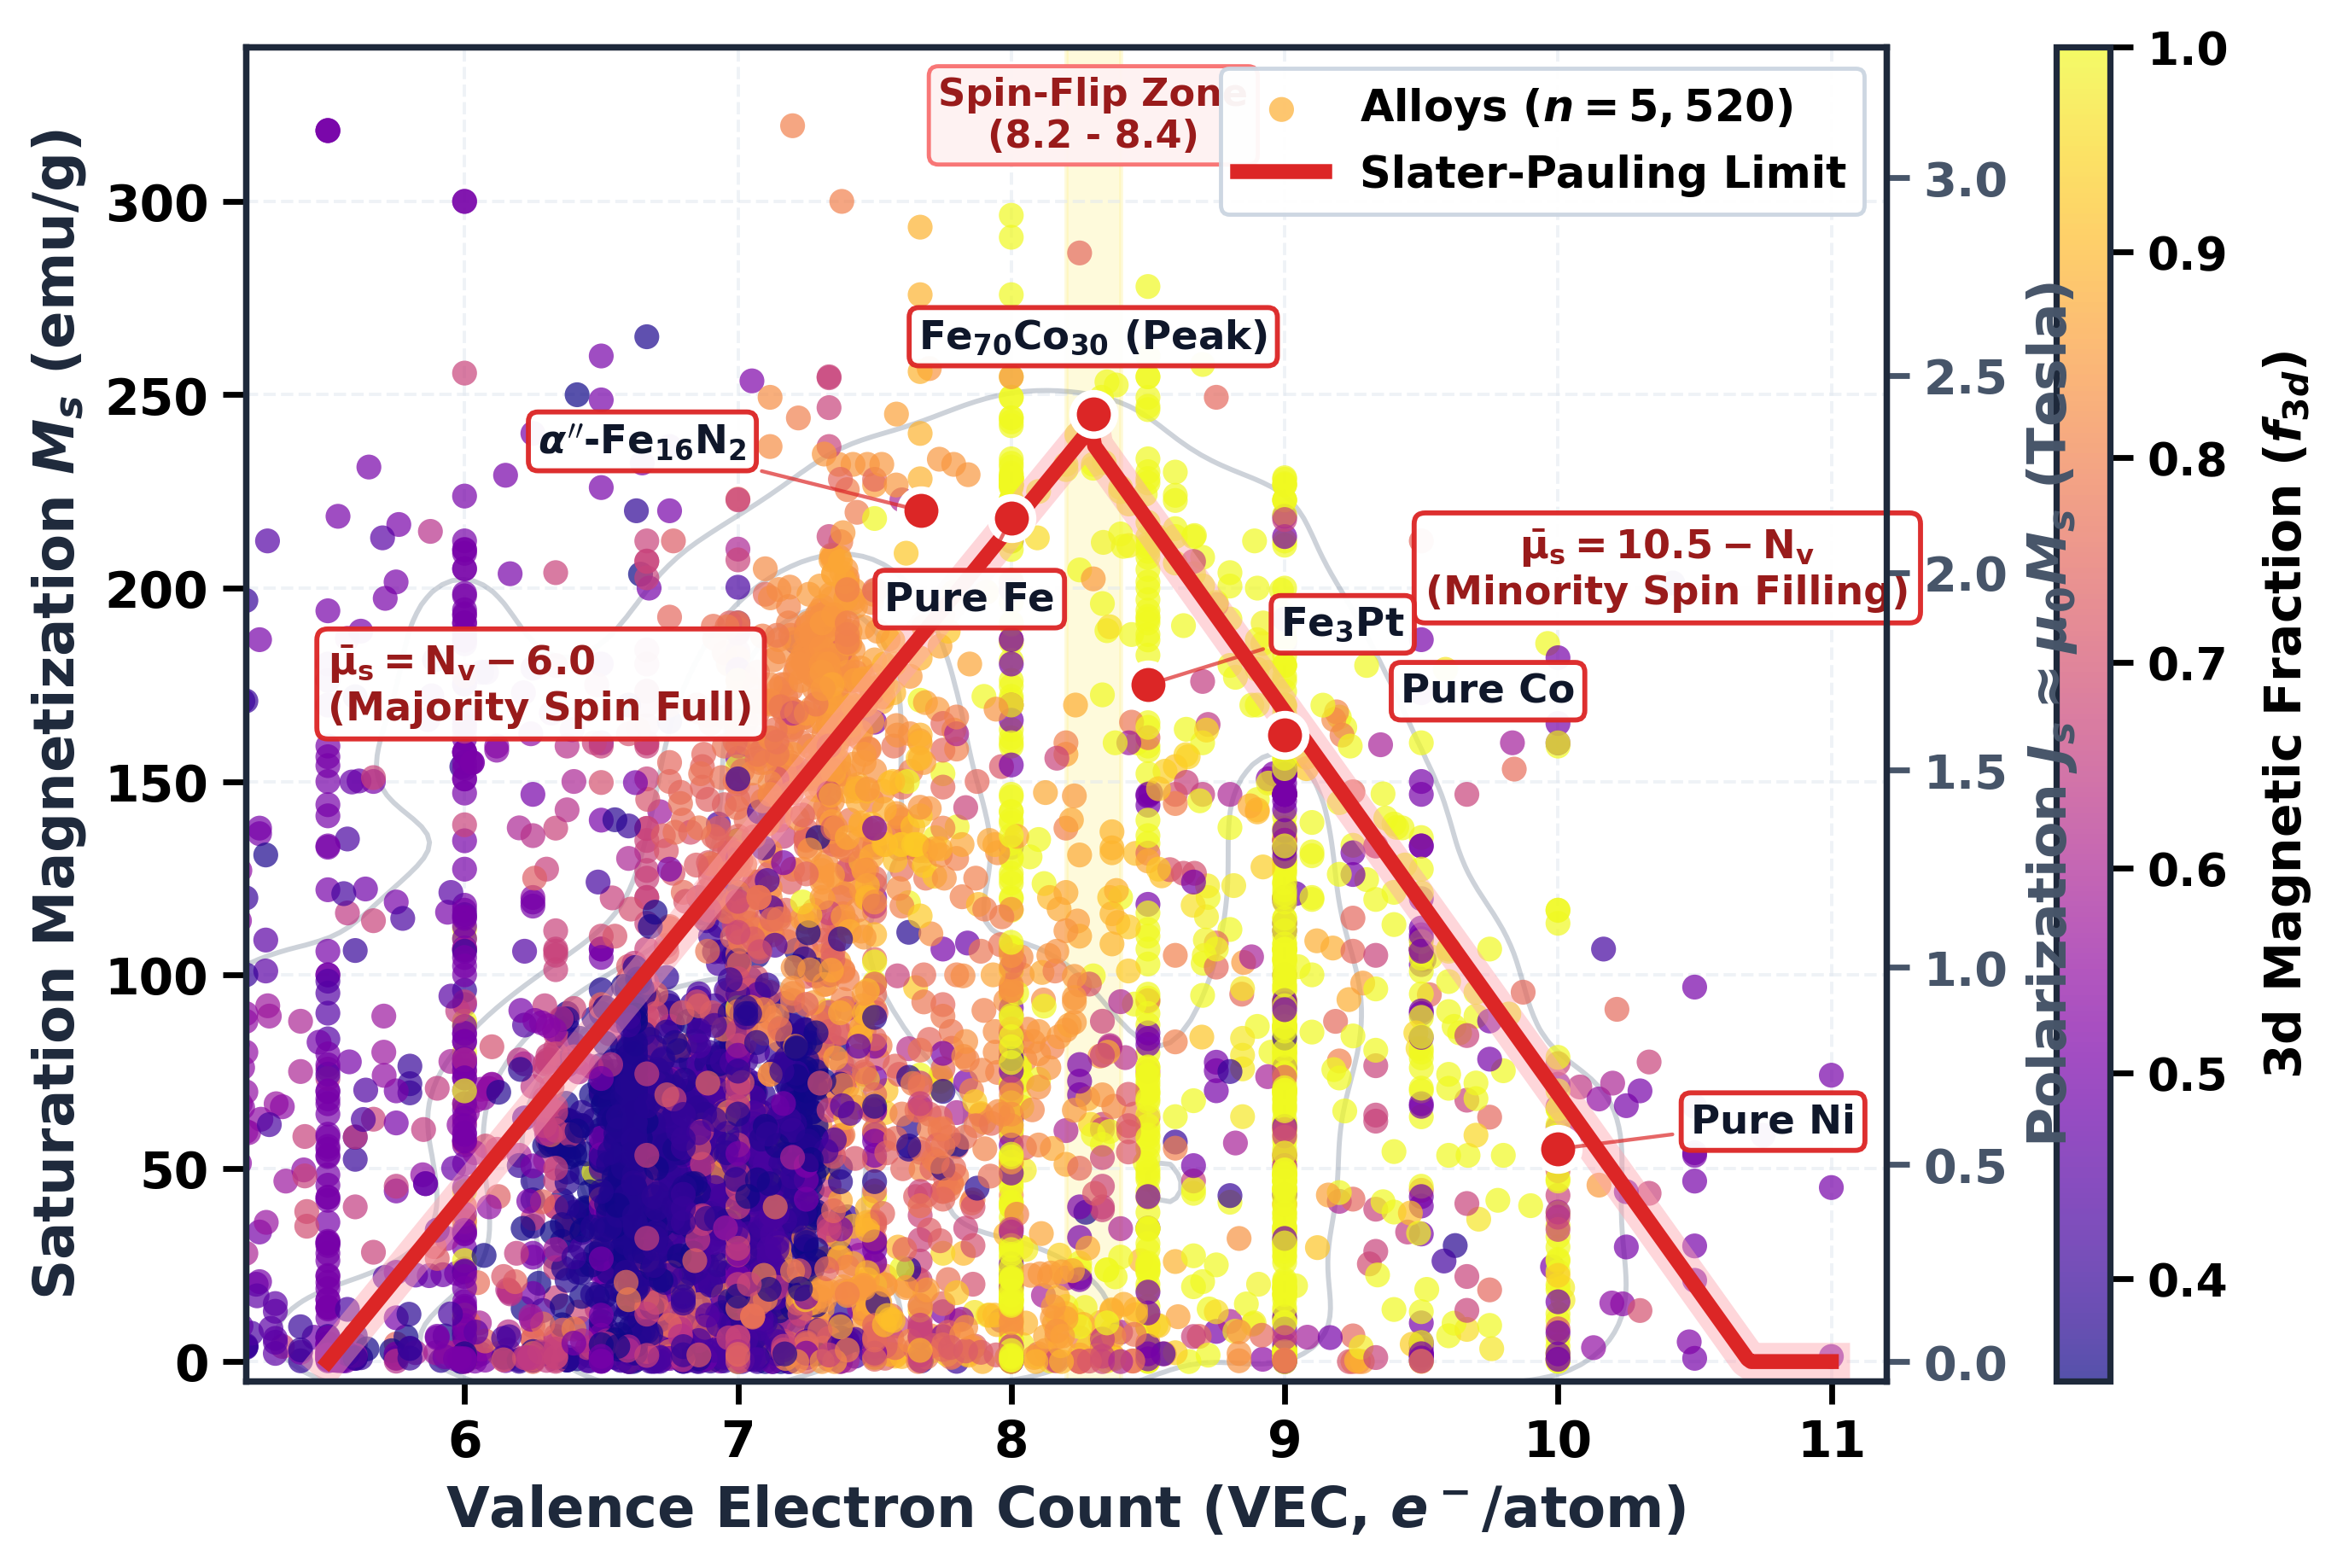
\includegraphics[width=0.82\textwidth]{figures/slater_pauling_curve.png}
  \vspace{-0.3em}
  \caption{\textbf{The Slater-Pauling Saturation Envelope.} Experimental alloy measurements (scatter points) sit beneath the theoretical rigid-band ceiling (red curve), peaking near $\text{VEC} \approx 8.25$ in Fe-Co ($2.45\,\mu_B$).}
  \label{fig:sp}
\end{figure}

\begin{takeawaybox}[Insight on Slater-Pauling]
The Slater-Pauling curve is an \textbf{upper bound, not a regressor}. Real materials scatter below the ceiling because spin canting, antiferromagnetic sub-lattices, and non-metallic bonding dilute net moments. A record appearing above this line is a diagnostic flag for bad or non-equilibrium experimental data.
\end{takeawaybox}

\subsection{Pillar 2: The 89\% Microstructural Defect Gap}
While saturation magnetization is an \emph{intrinsic property} determined by composition, coercivity ($H_c$) is an \emph{extrinsic property} governed by microstructure, grain boundaries, and crystal defects.

\begin{figure}[htbp]
  \centering
  \begin{subfigure}[b]{0.48\textwidth}
    \centering
    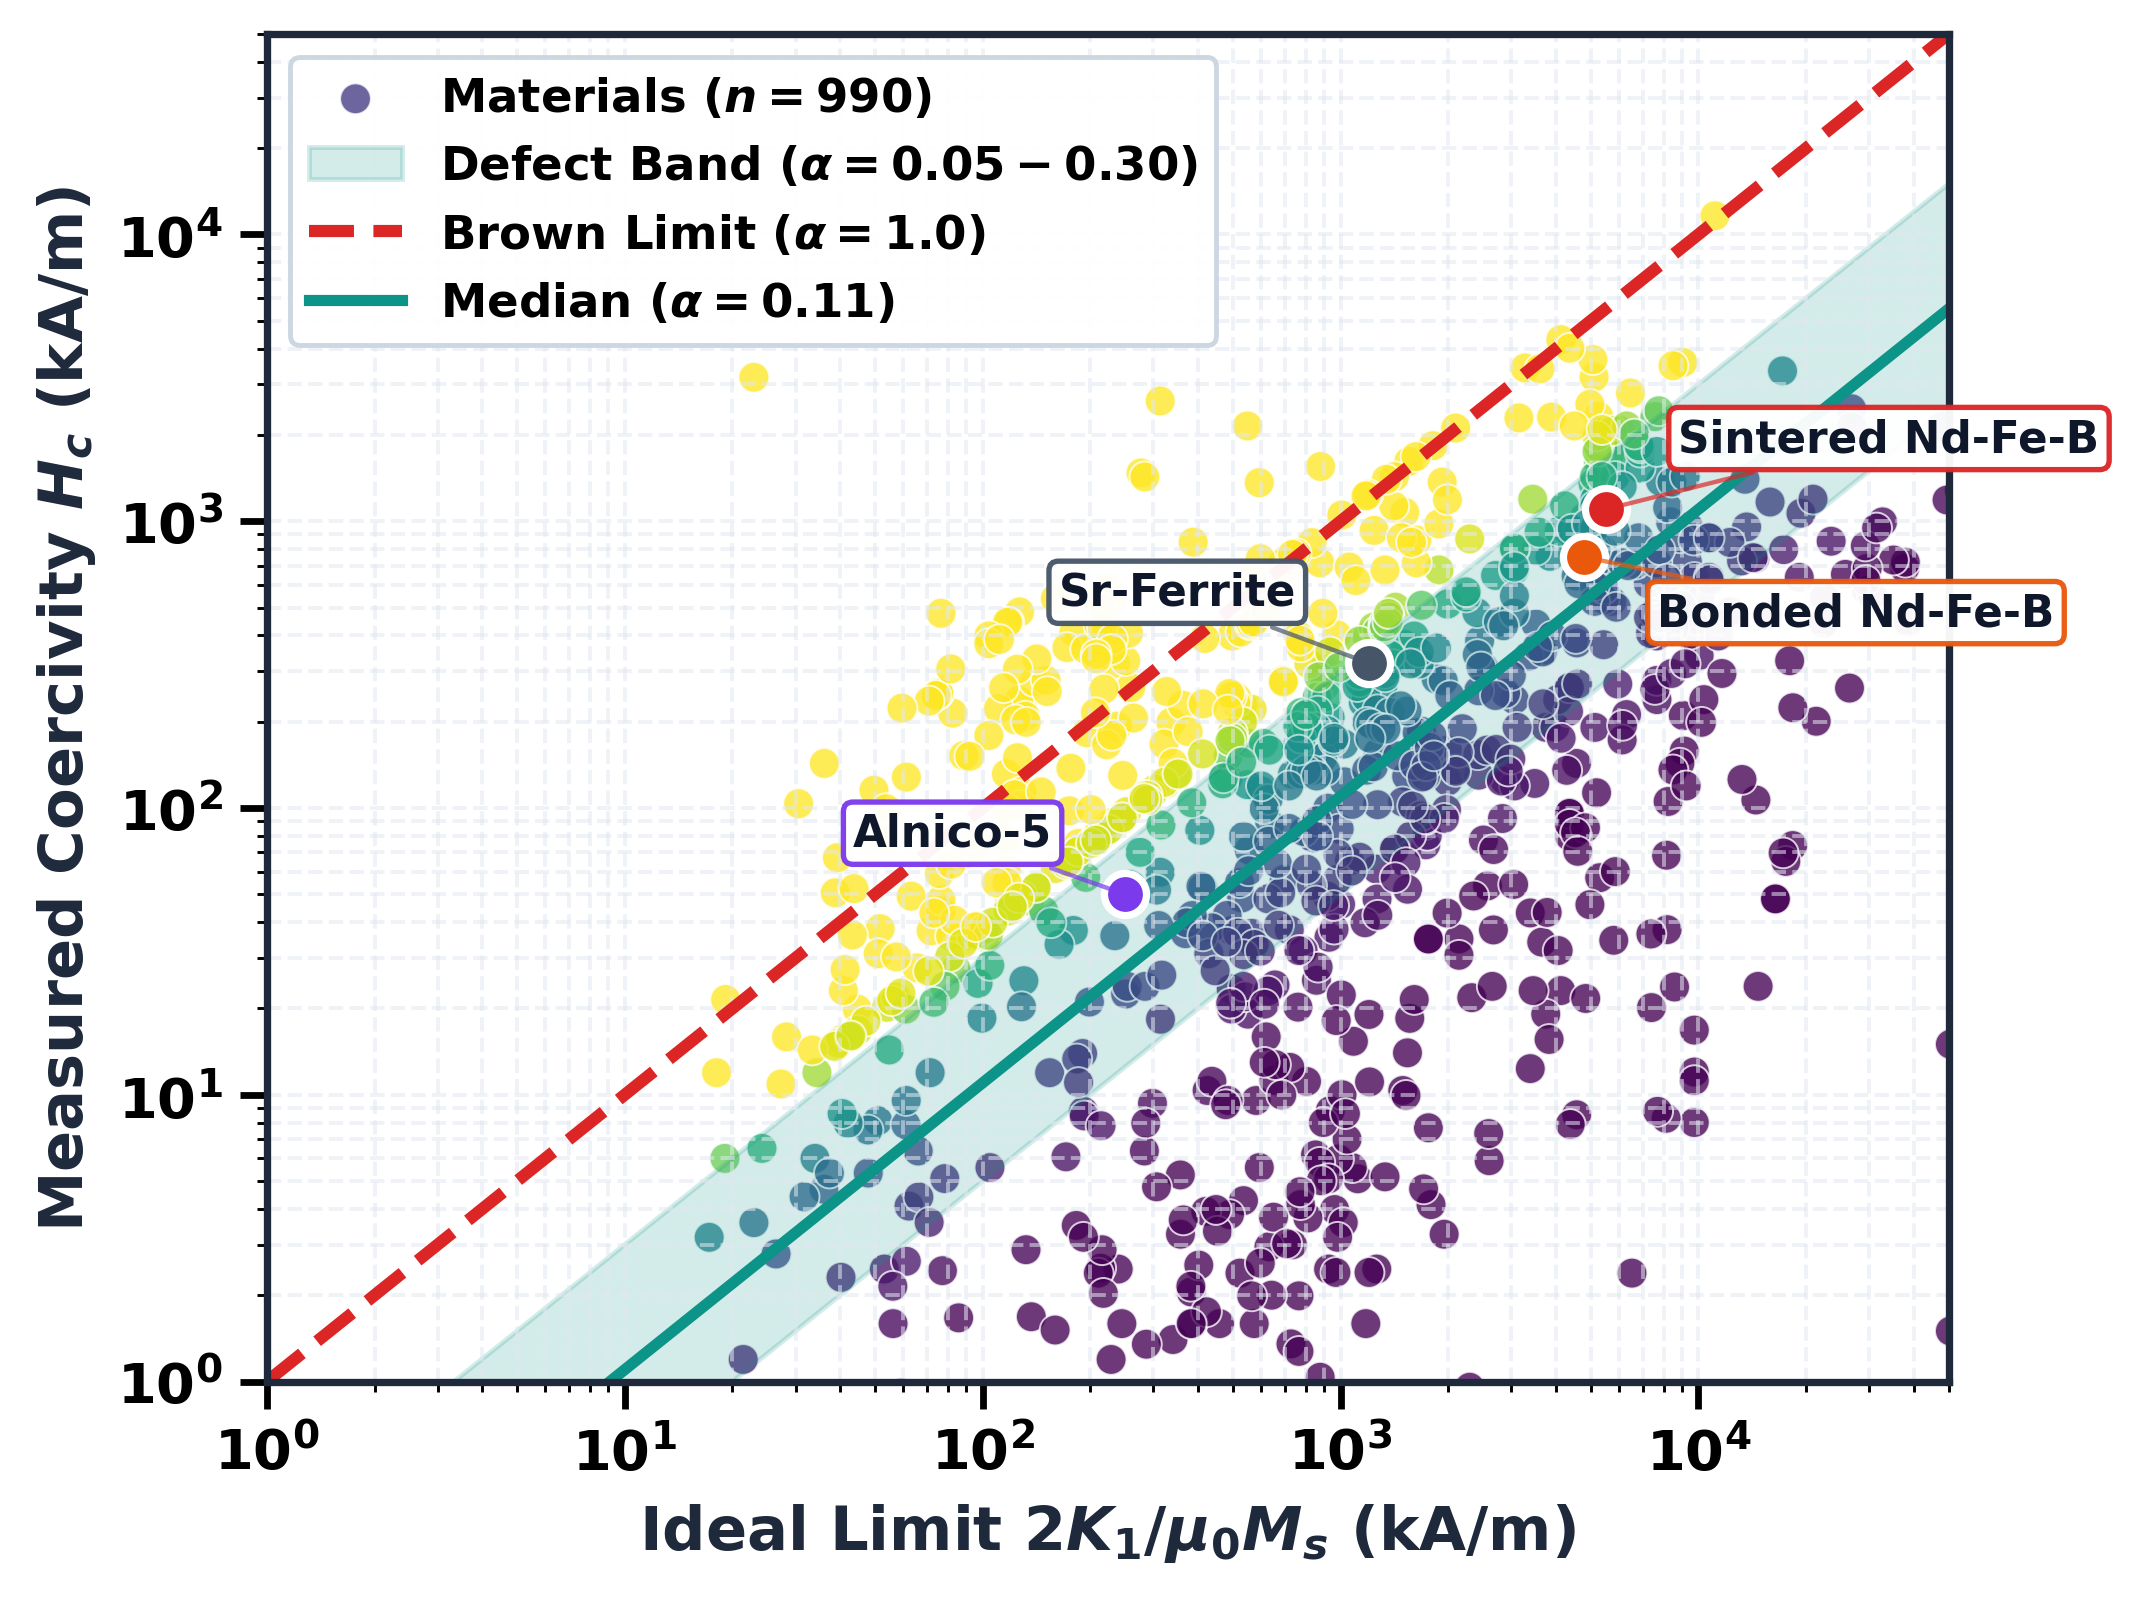
\includegraphics[width=\textwidth]{figures/kronmuller_scatter.png}
    \caption{Realized $H_c$ vs.\ Ideal Nucleation Limit $H_K$}
  \end{subfigure}
  \hfill
  \begin{subfigure}[b]{0.48\textwidth}
    \centering
    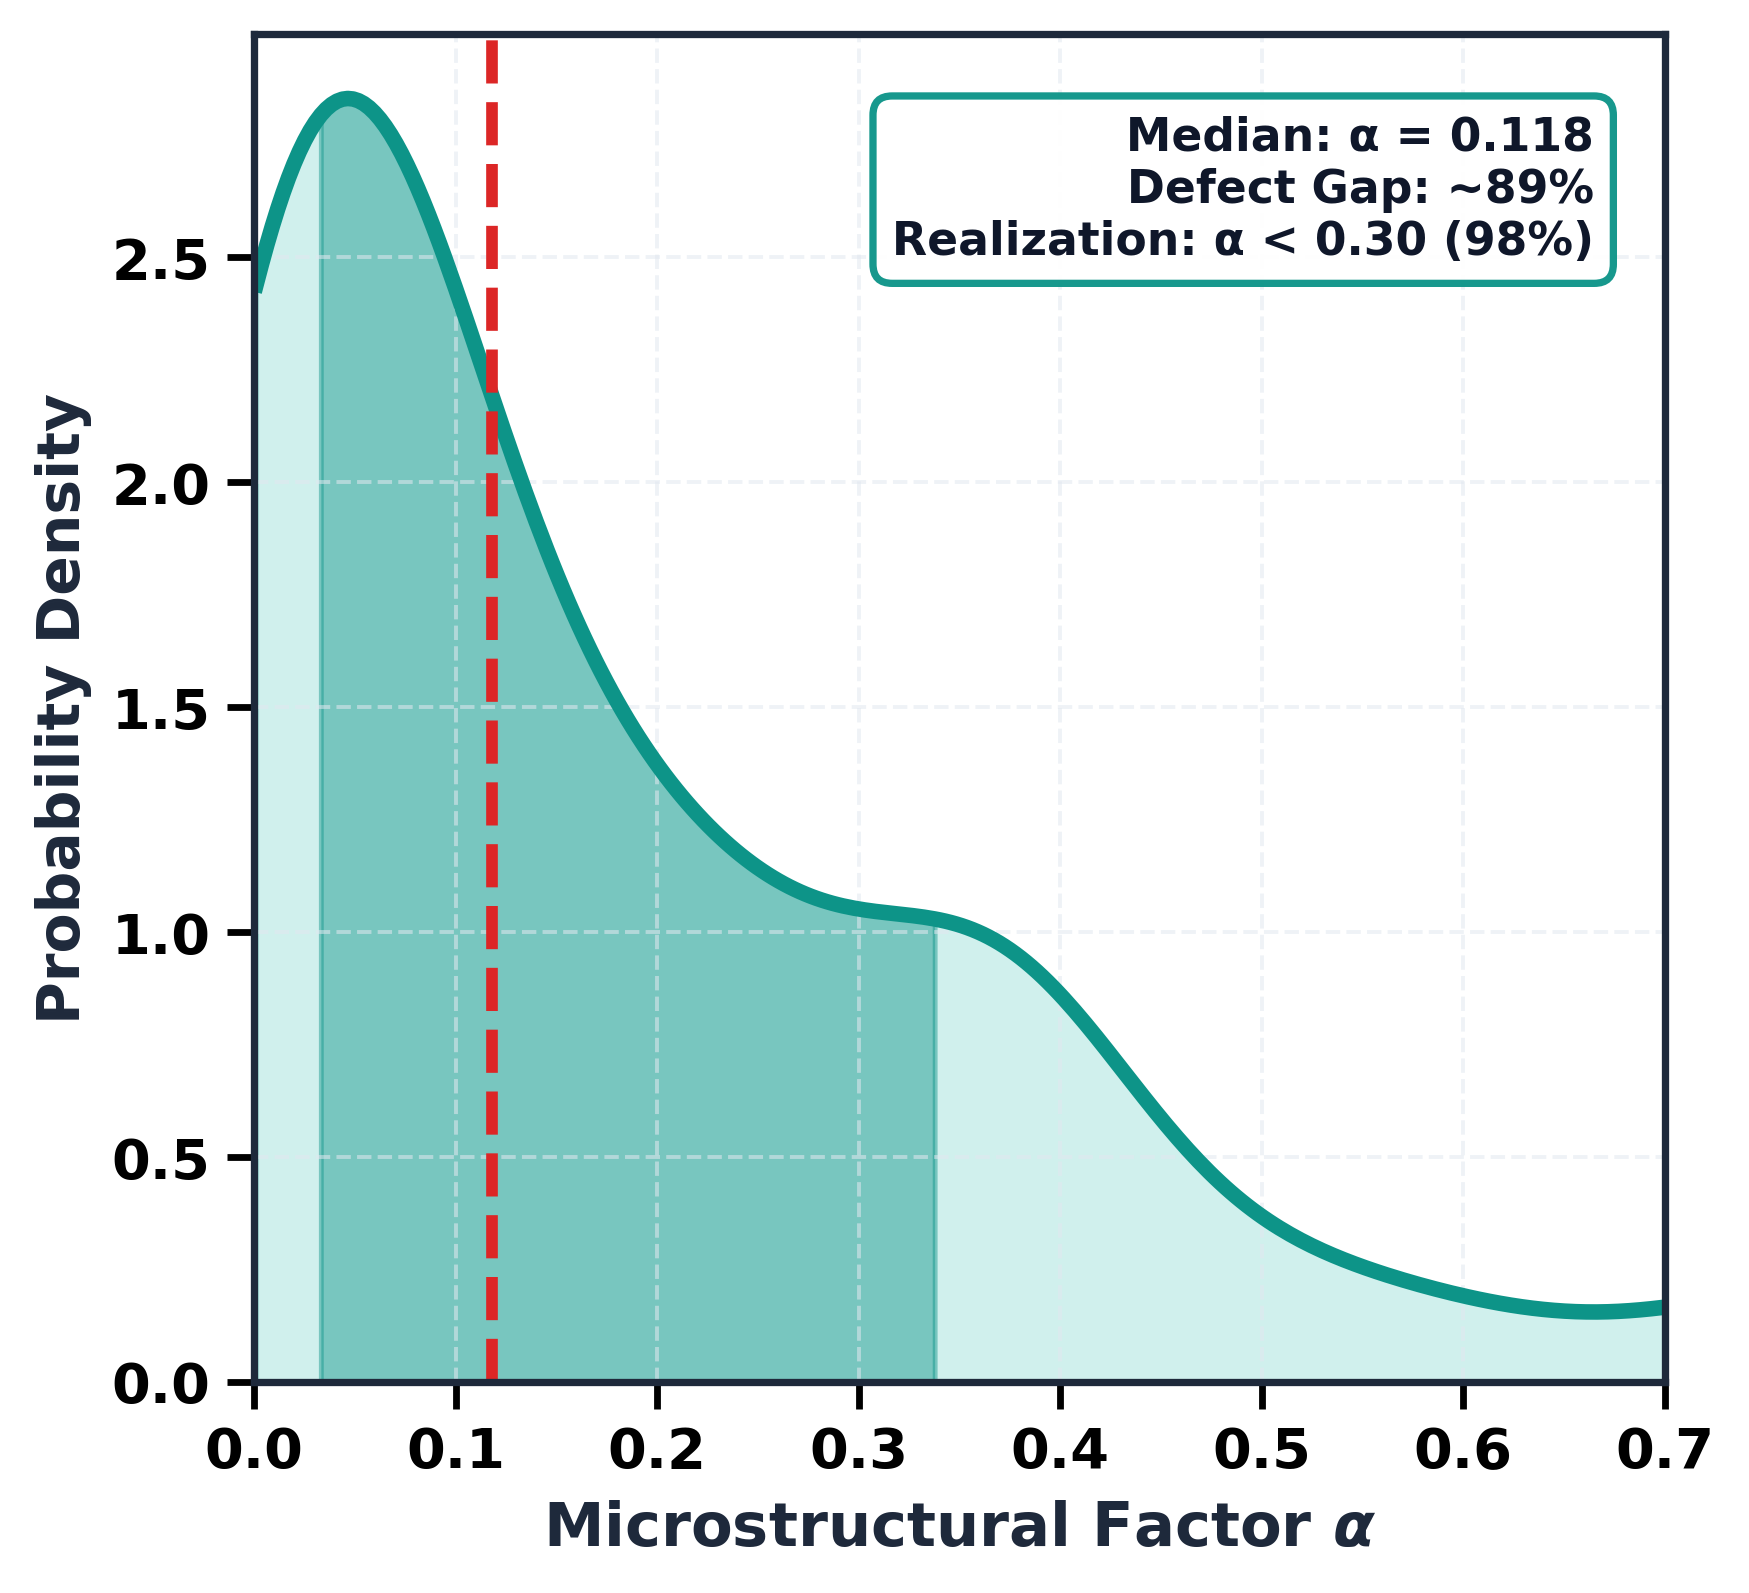
\includegraphics[width=\textwidth]{figures/kronmuller_defect_hist.png}
    \caption{Distribution of Realization Factor $\alpha = H_c / H_K$}
  \end{subfigure}
  \vspace{-0.3em}
  \caption{\textbf{The Microstructural Coercivity Gap.} (a) Experimental magnets sit one to two orders of magnitude below Brown's ideal limit. (b) The median realization factor across 1,064 records is $\alpha \approx 0.118$, demonstrating an $89\%$ defect gap.}
  \label{fig:kronmuller}
\end{figure}

\begin{takeawaybox}[Why 3D Structural AI is Essential]
In real sintered magnets, local grain misorientations and defect sites nucleate reverse magnetic domains at fields far below the ideal single-crystal limit ($H_c \approx \alpha \frac{2K_1}{\mu_0 M_s}$). Because this missing 89\% headroom lives in geometry rather than chemical formulas, predicting coercivity requires \textbf{3D atomistic representations} provided by foundation AI models (DAO and MACE).
\end{takeawaybox}

% =========================================================================
\section{Harmonized Experimental Data Landscape (56,781 Records)}
% =========================================================================

The dataset integrates 56,781 experimental measurements from NEMAD, Landolt-Börnstein handbooks, and primary literature covering eight core magnetic properties.

\begin{figure}[htbp]
  \centering
  \begin{subfigure}[b]{0.48\textwidth}
    \centering
    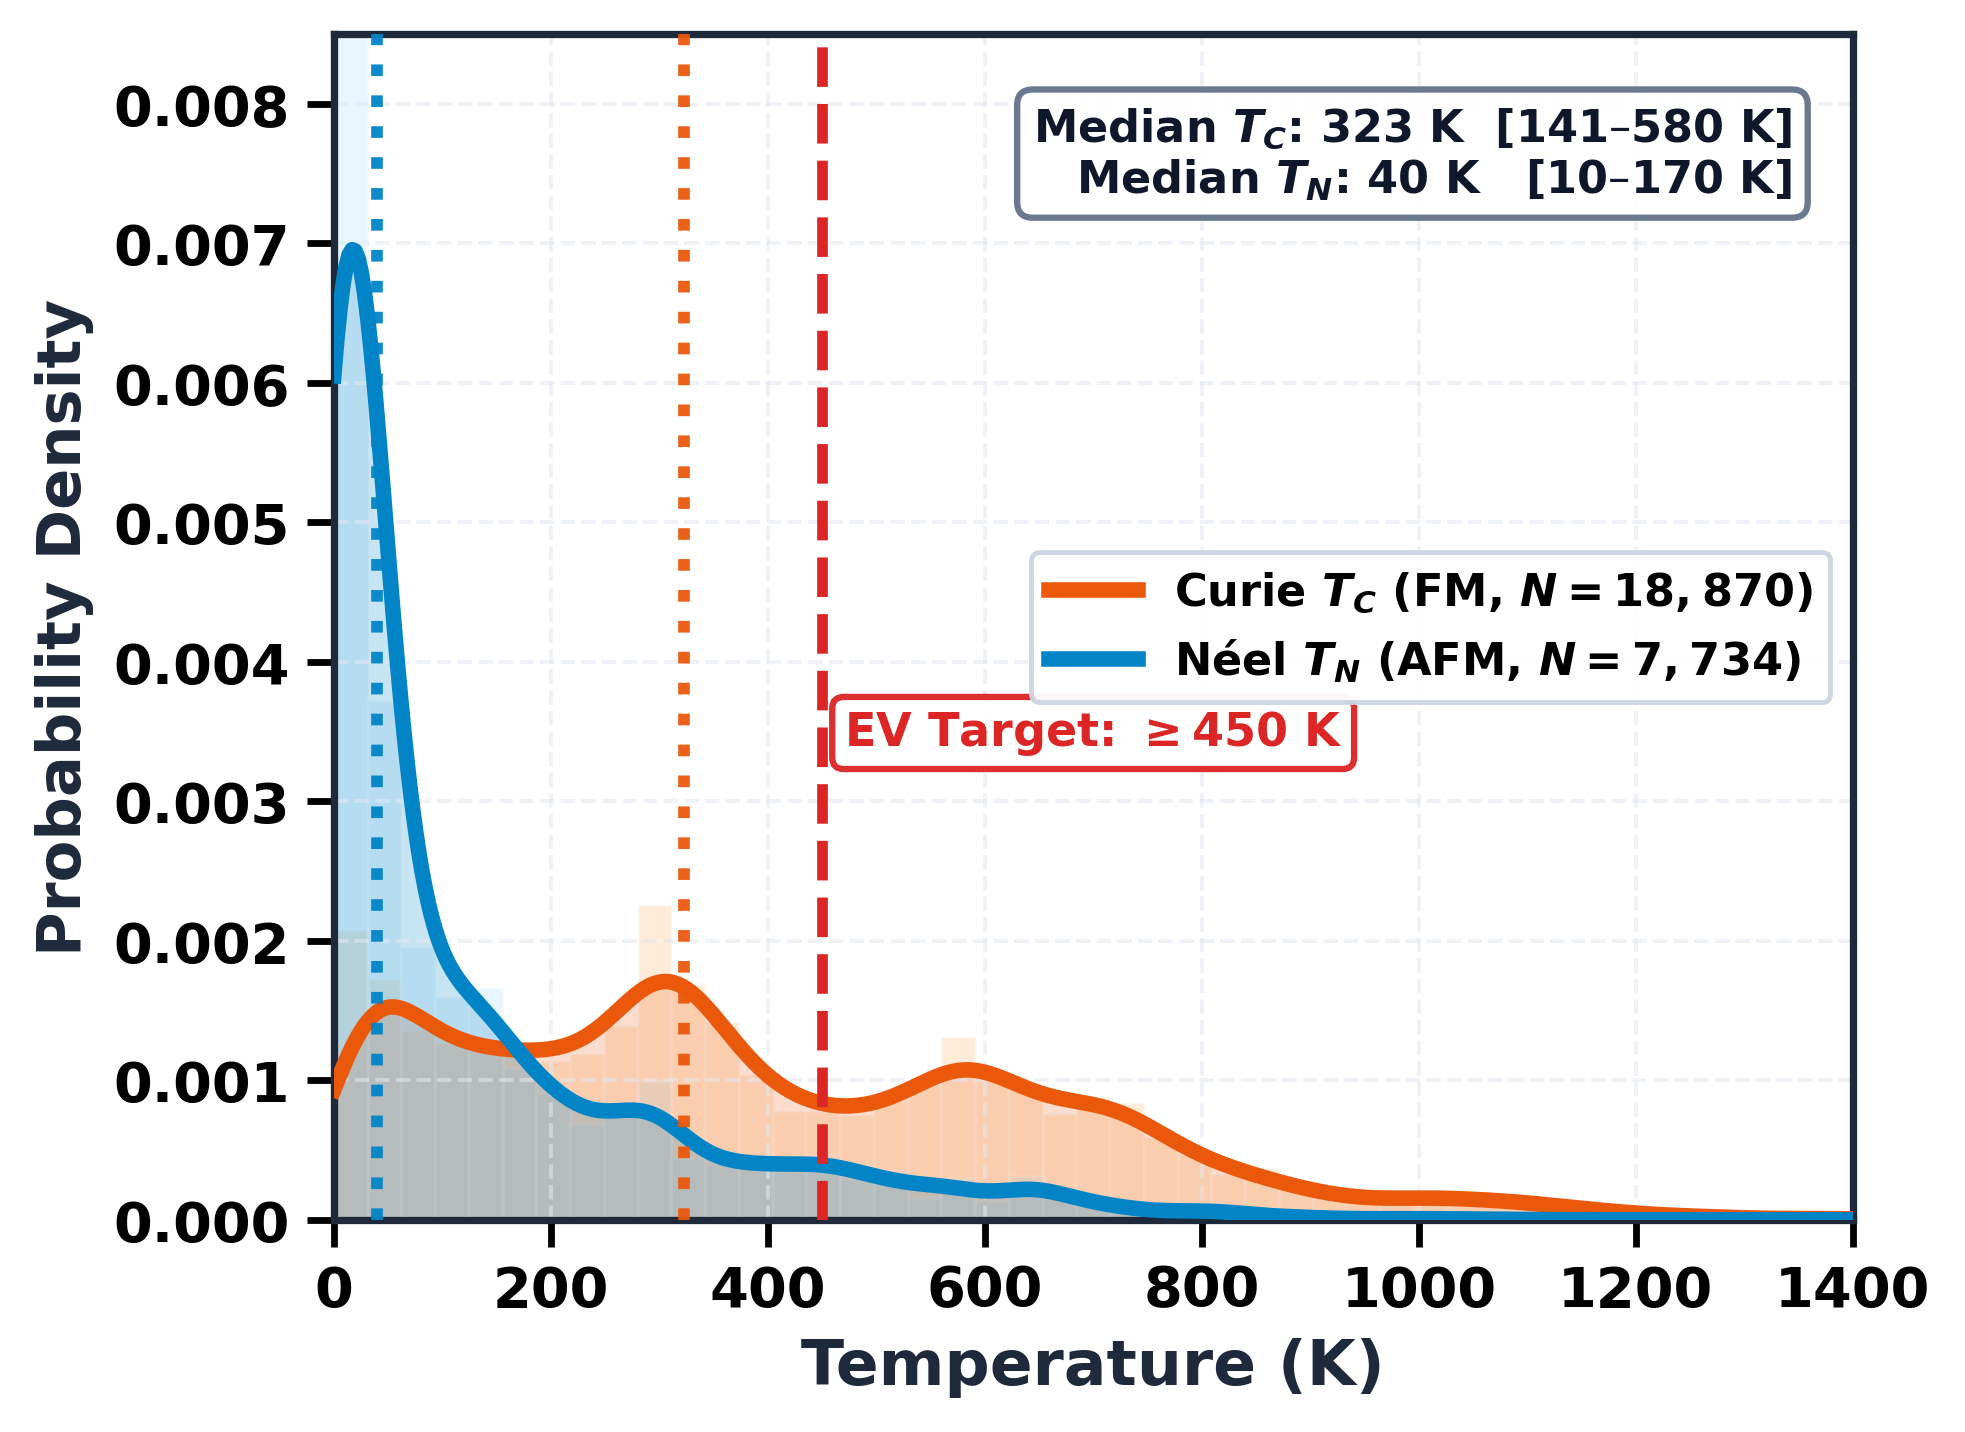
\includegraphics[width=\textwidth]{figures/dist_tc_tn.png}
    \caption{Curie ($T_C$) and Néel ($T_N$) Temperatures}
  \end{subfigure}
  \hfill
  \begin{subfigure}[b]{0.48\textwidth}
    \centering
    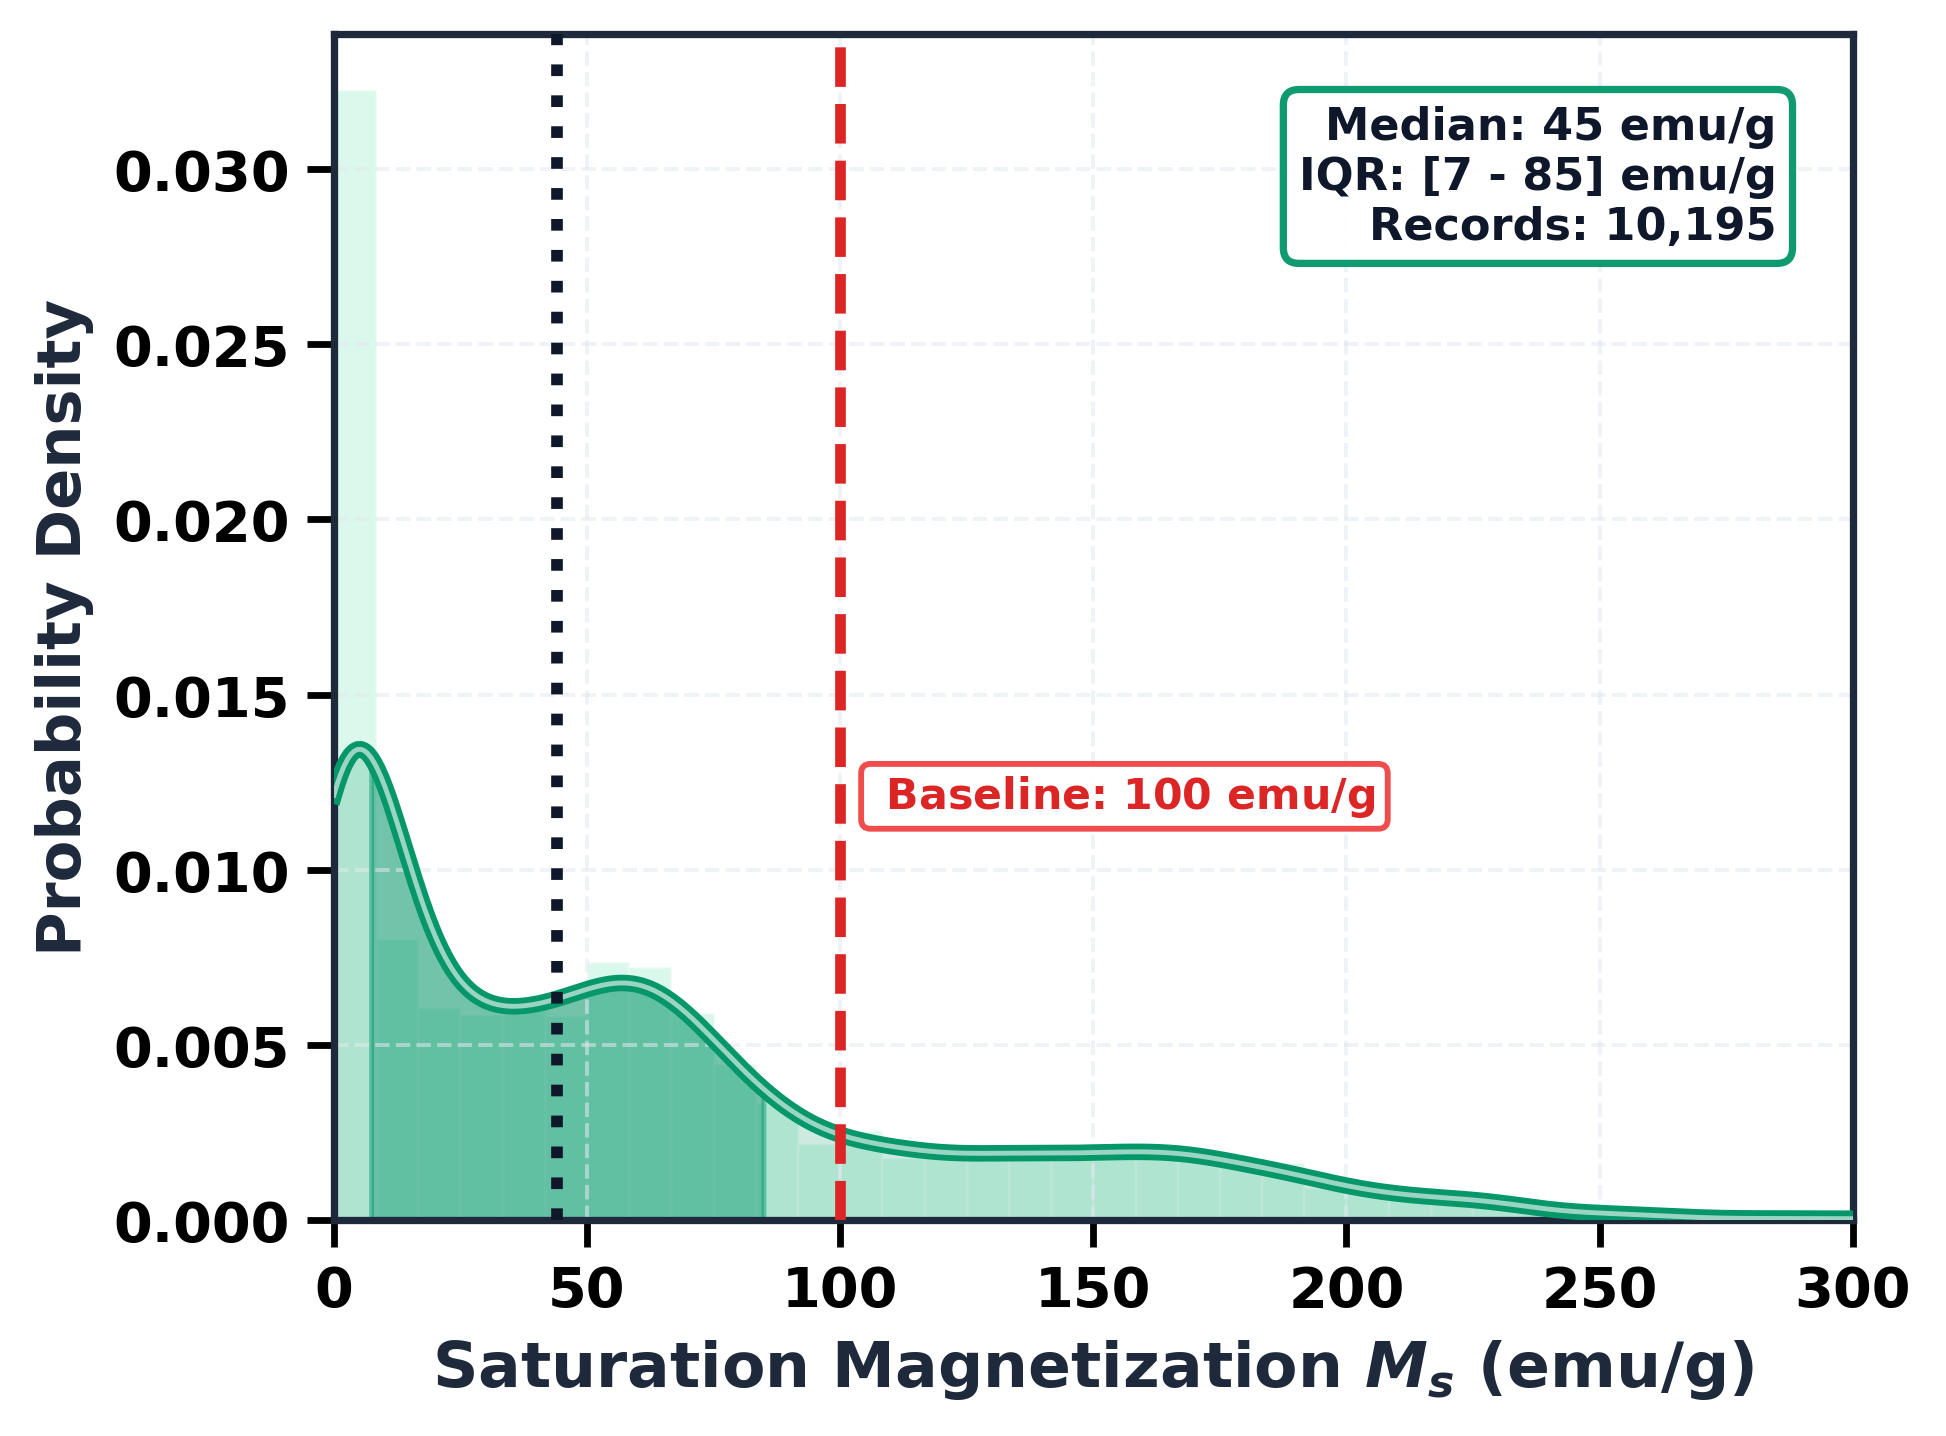
\includegraphics[width=\textwidth]{figures/dist_ms.png}
    \caption{Saturation Magnetization ($M_s$)}
  \end{subfigure}
  
  \vspace{0.4em}
  \begin{subfigure}[b]{0.48\textwidth}
    \centering
    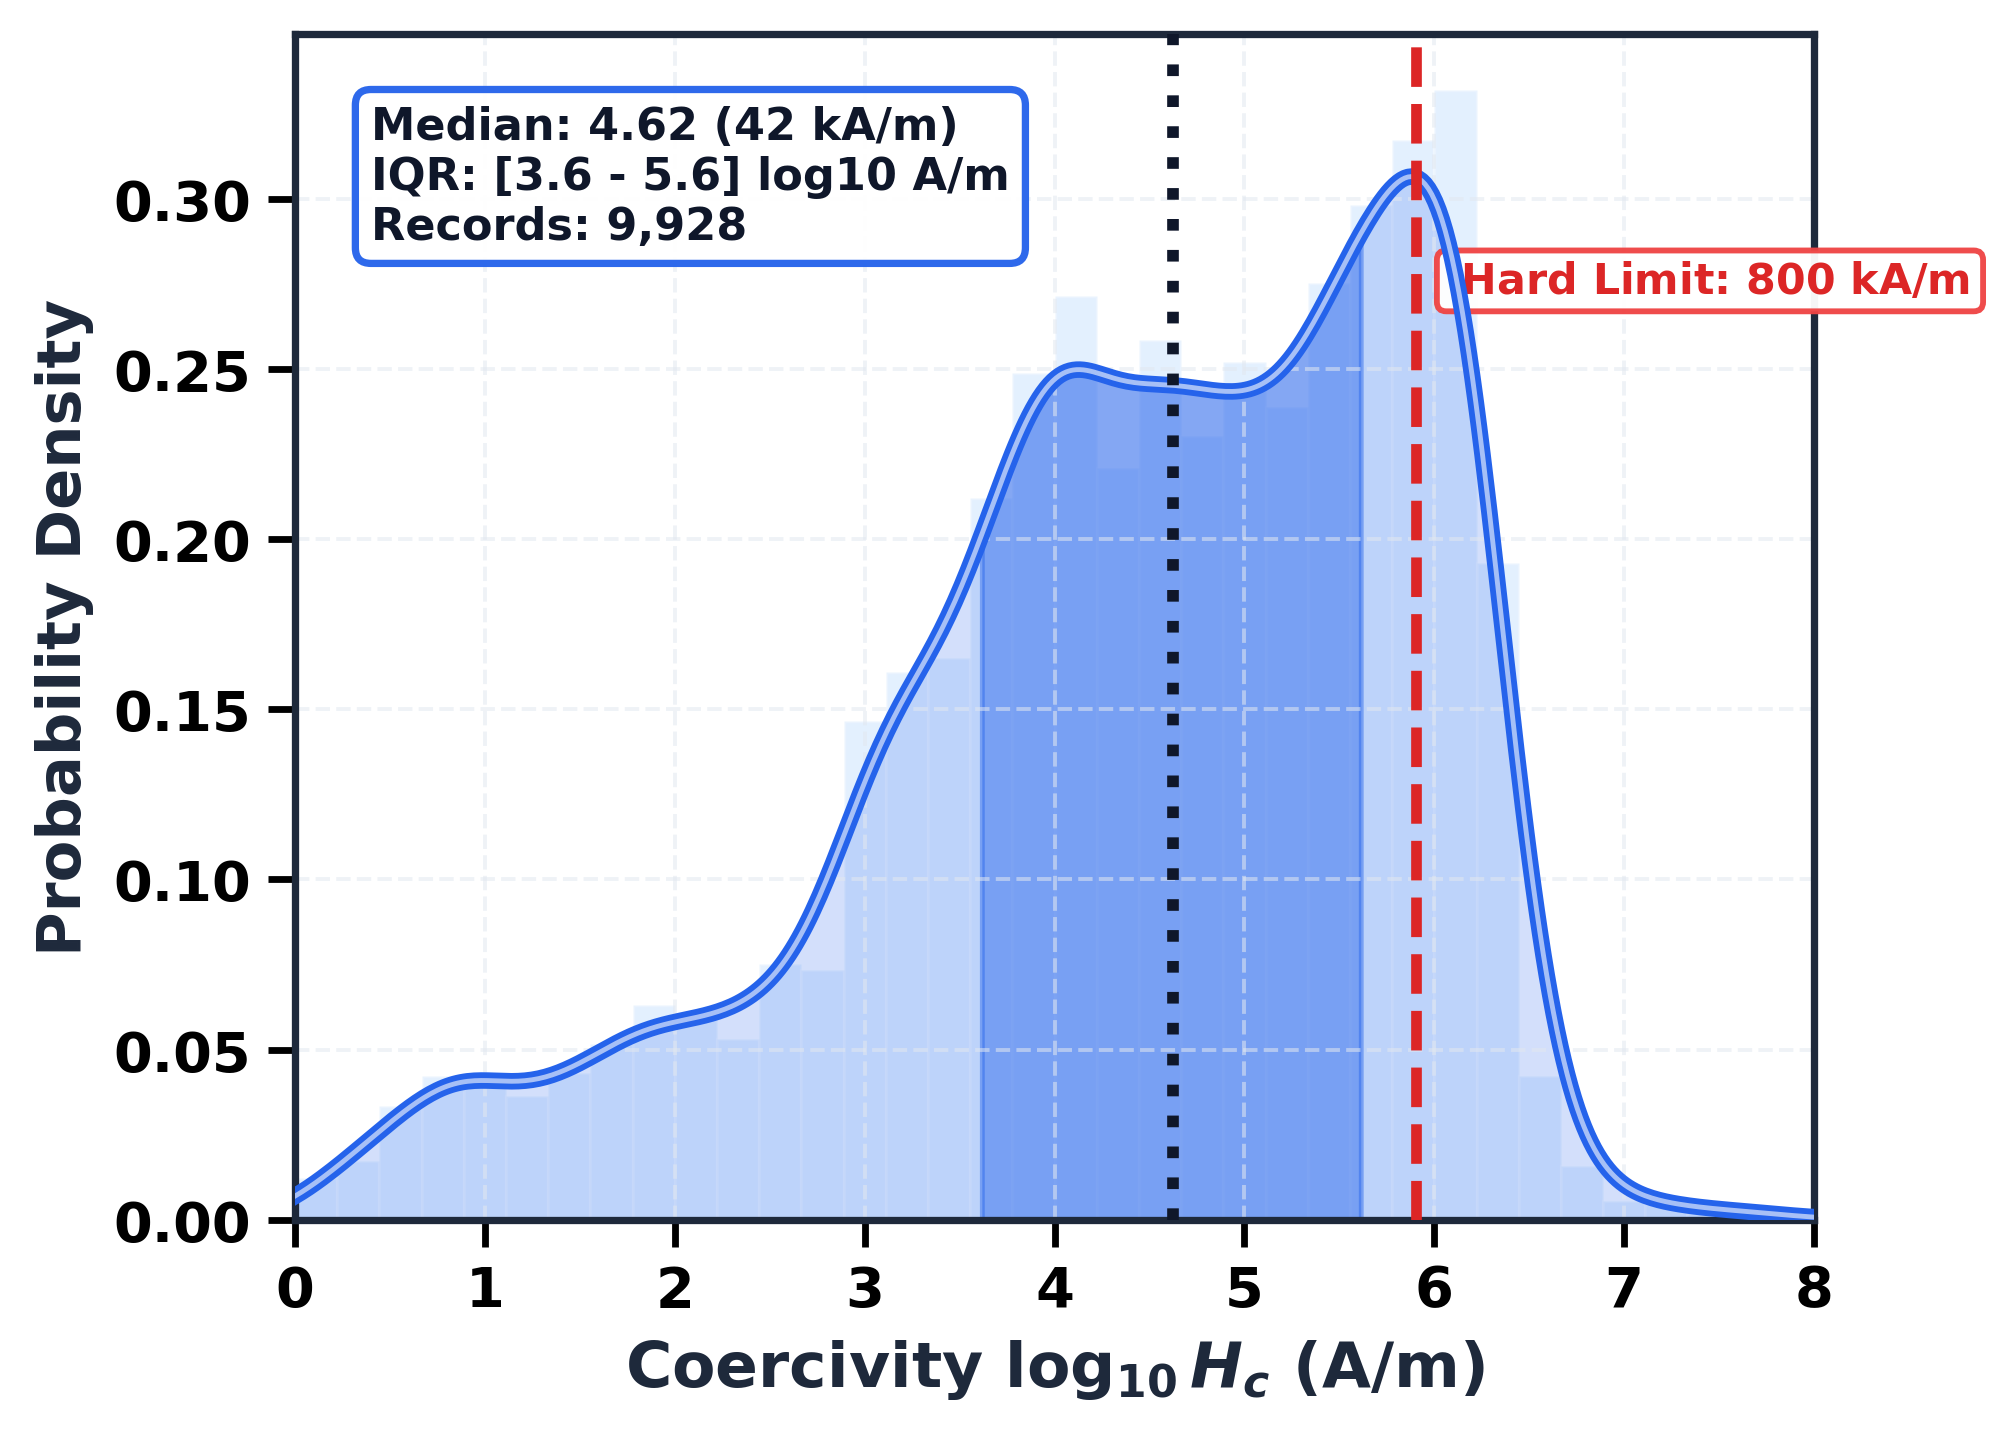
\includegraphics[width=\textwidth]{figures/dist_hc.png}
    \caption{Coercive Field ($\log_{10} H_c$)}
  \end{subfigure}
  \hfill
  \begin{subfigure}[b]{0.48\textwidth}
    \centering
    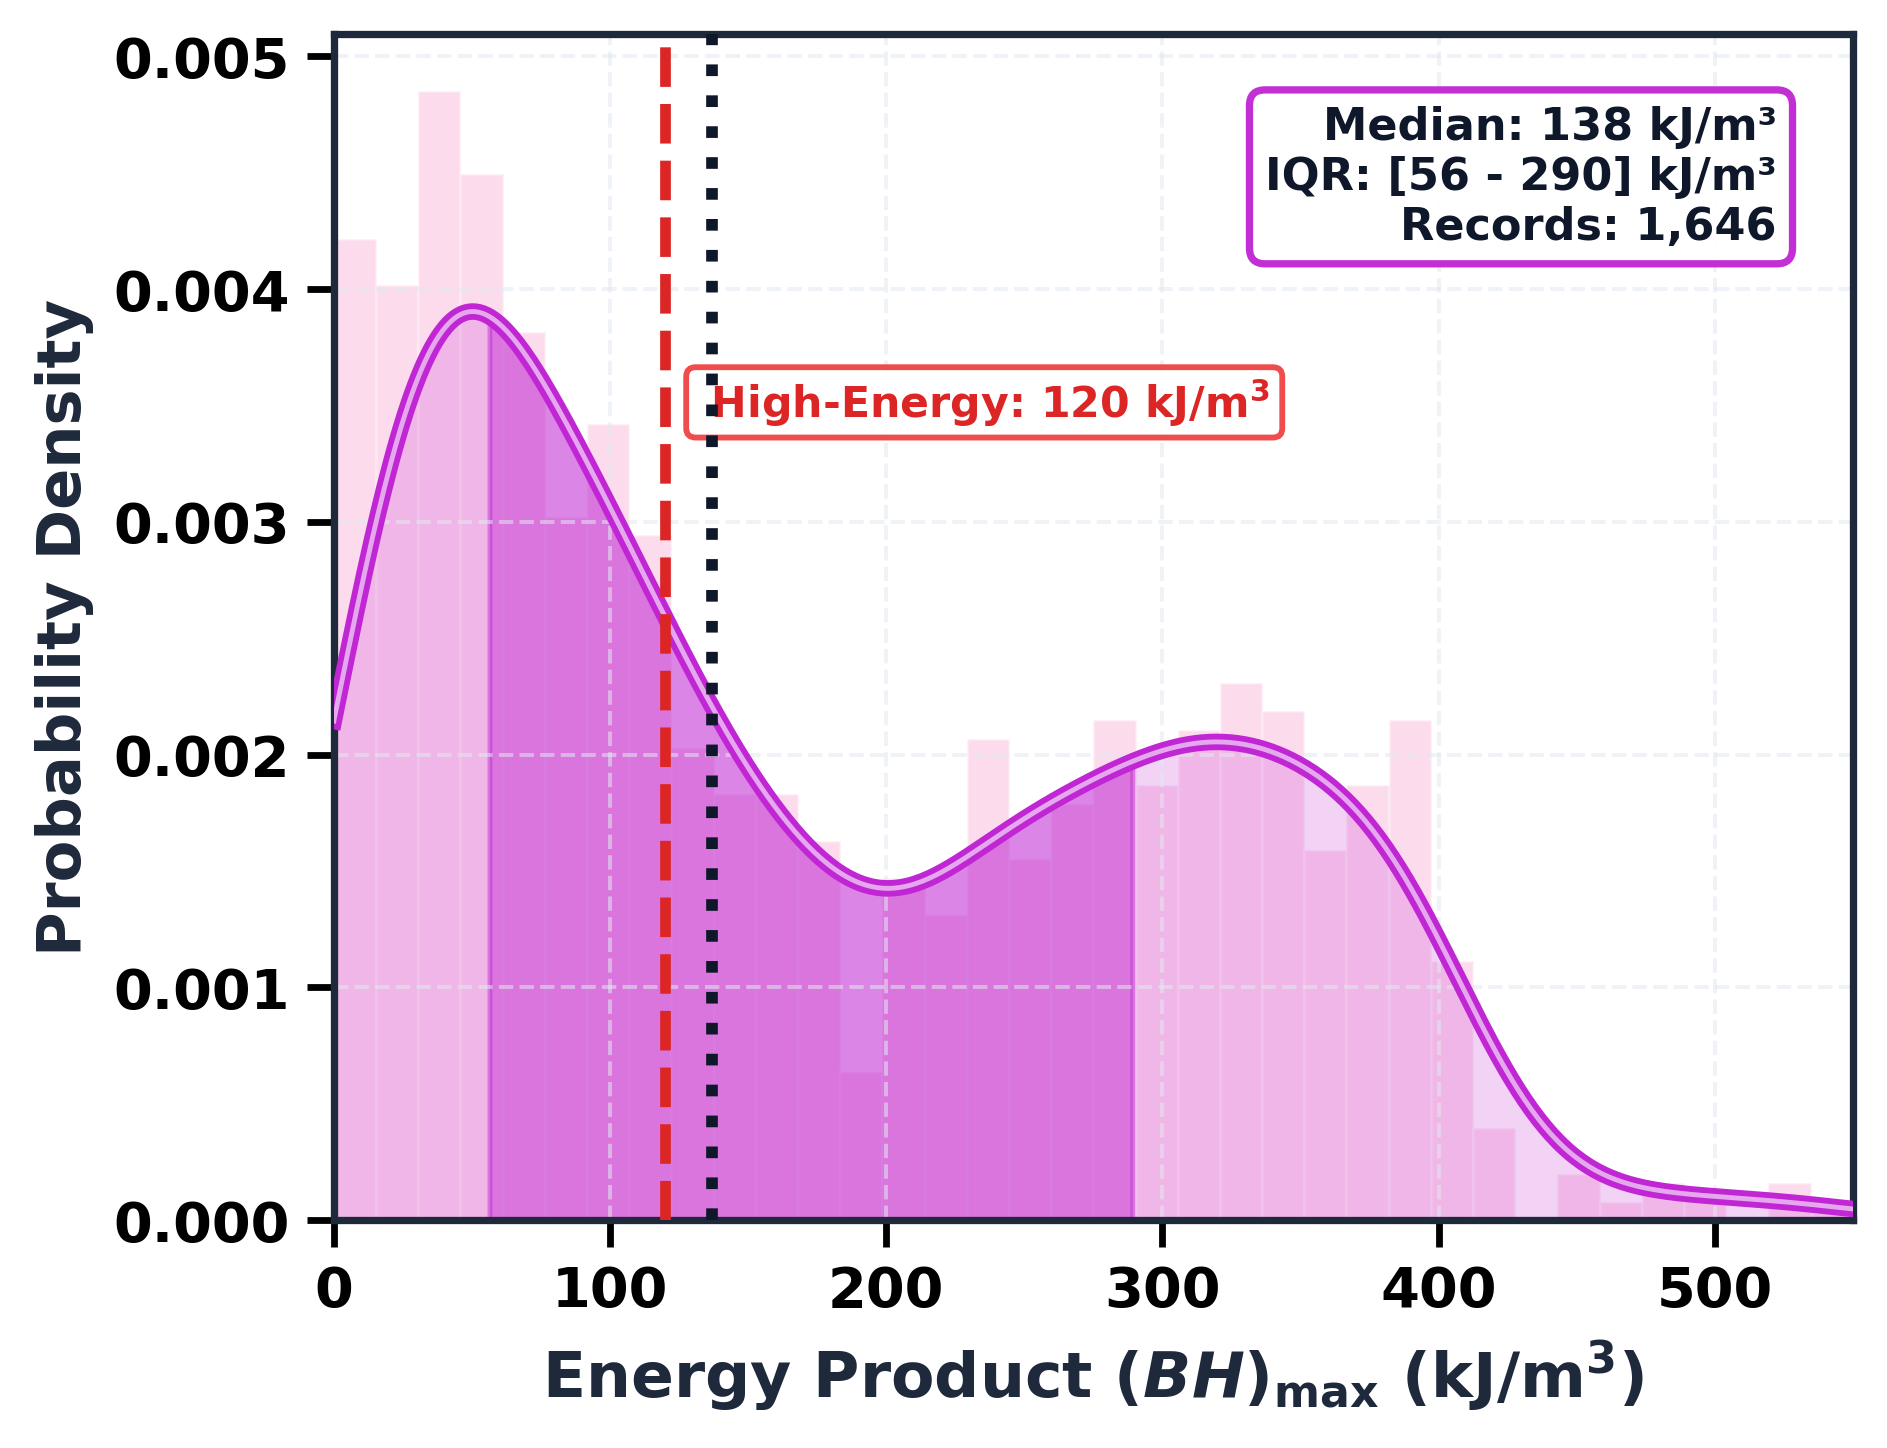
\includegraphics[width=\textwidth]{figures/dist_bhmax.png}
    \caption{Maximum Energy Product ($(BH)_{\max}$)}
  \end{subfigure}
  \vspace{-0.3em}
  \caption{\textbf{Empirical Distributions of Core Magnetic Properties.} Showing broad dynamic ranges, multi-modal transition temperatures, and wide coercivity spans across experimental materials.}
  \label{fig:dists}
\end{figure}

\subsection{Correlation Drivers of Magnetism}
\begin{figure}[htbp]
  \centering
  \begin{subfigure}[b]{0.48\textwidth}
    \centering
    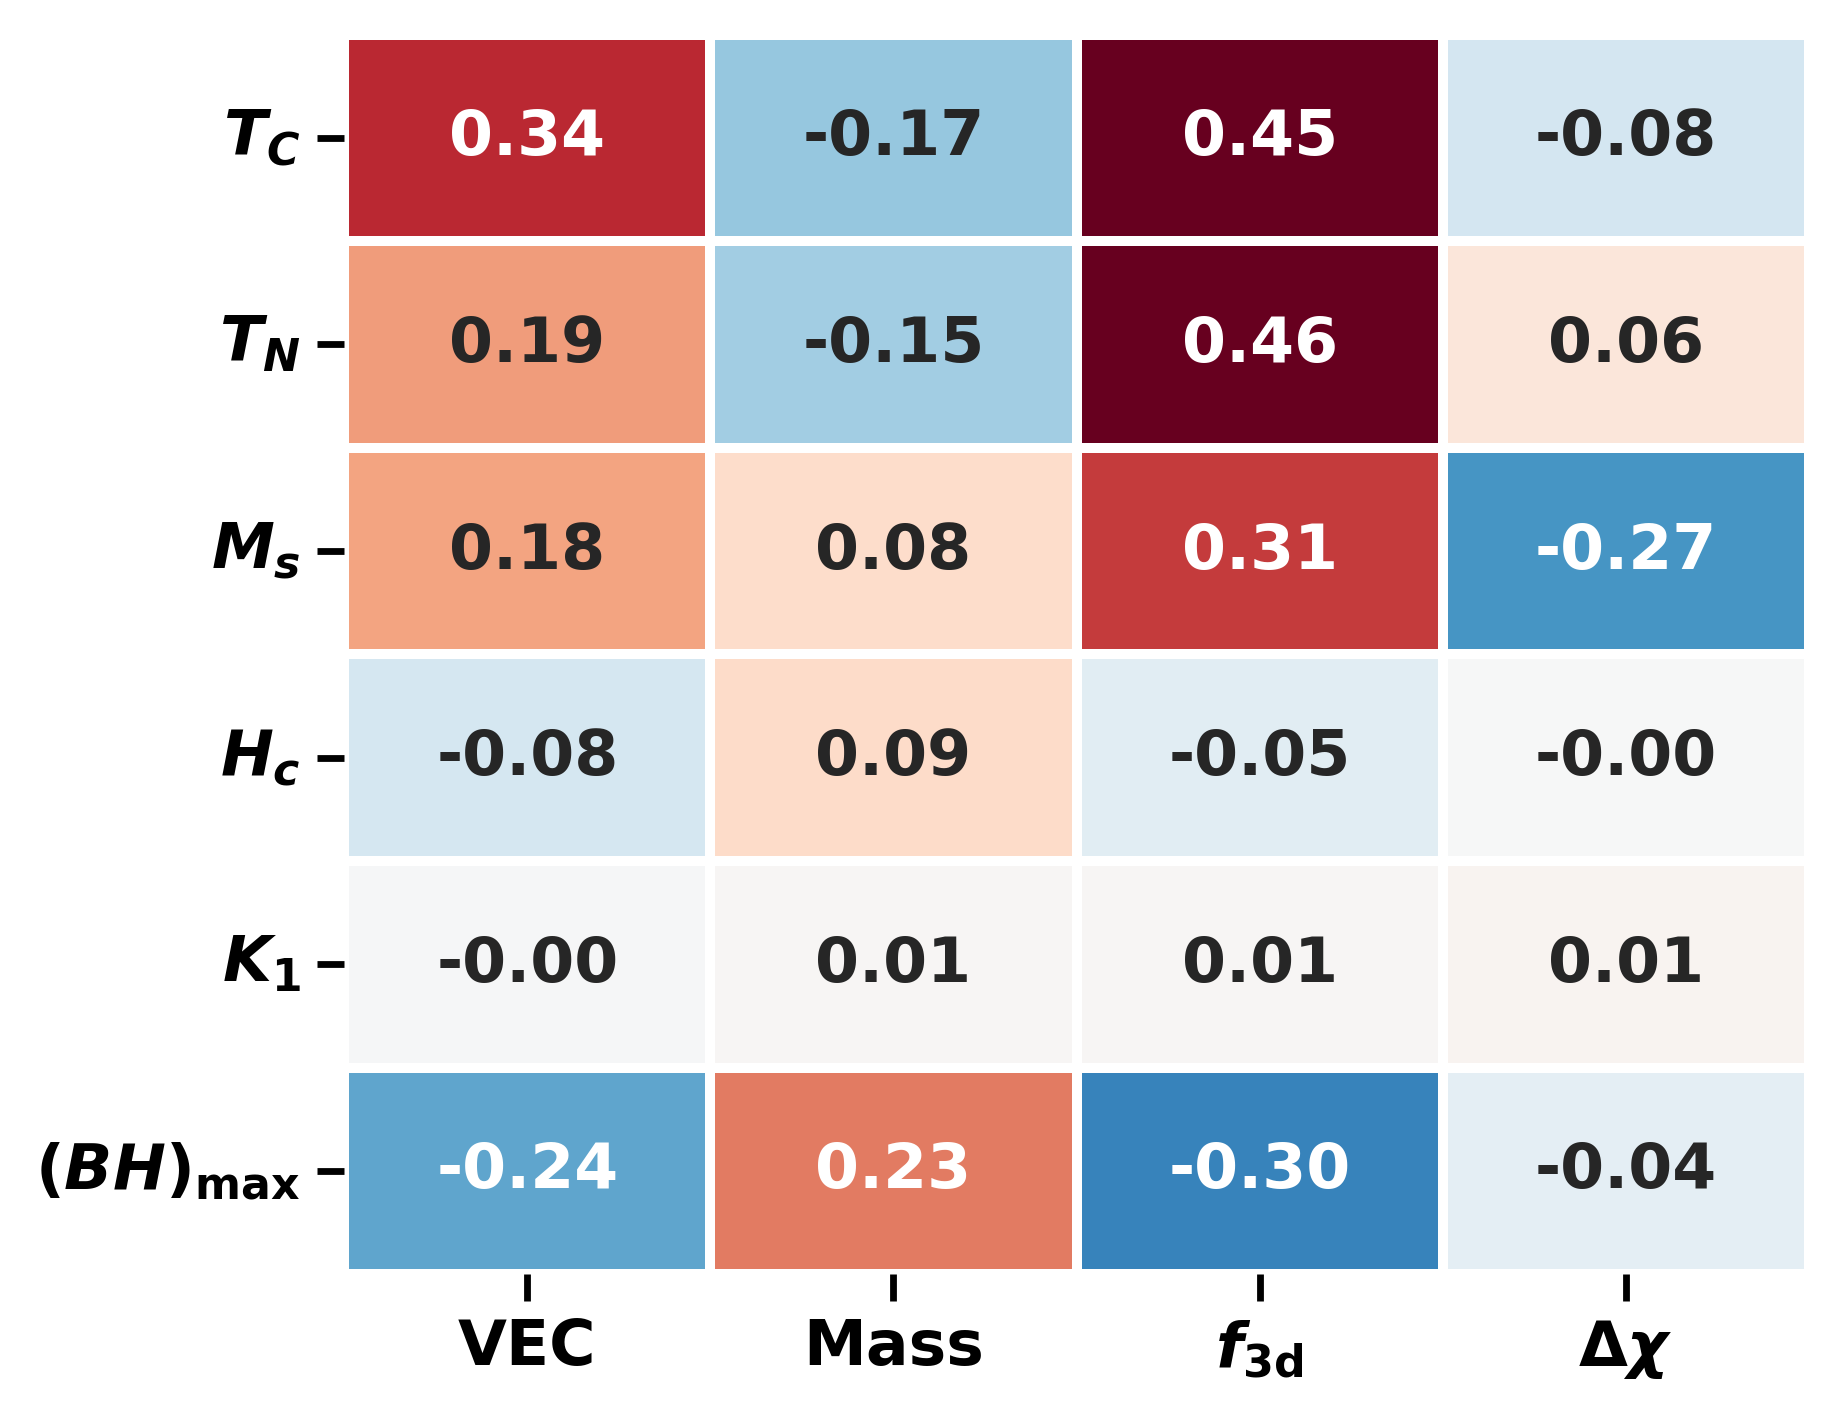
\includegraphics[width=\textwidth]{figures/corr_pearson.png}
    \caption{Pearson Linear Correlation ($r$)}
  \end{subfigure}
  \hfill
  \begin{subfigure}[b]{0.48\textwidth}
    \centering
    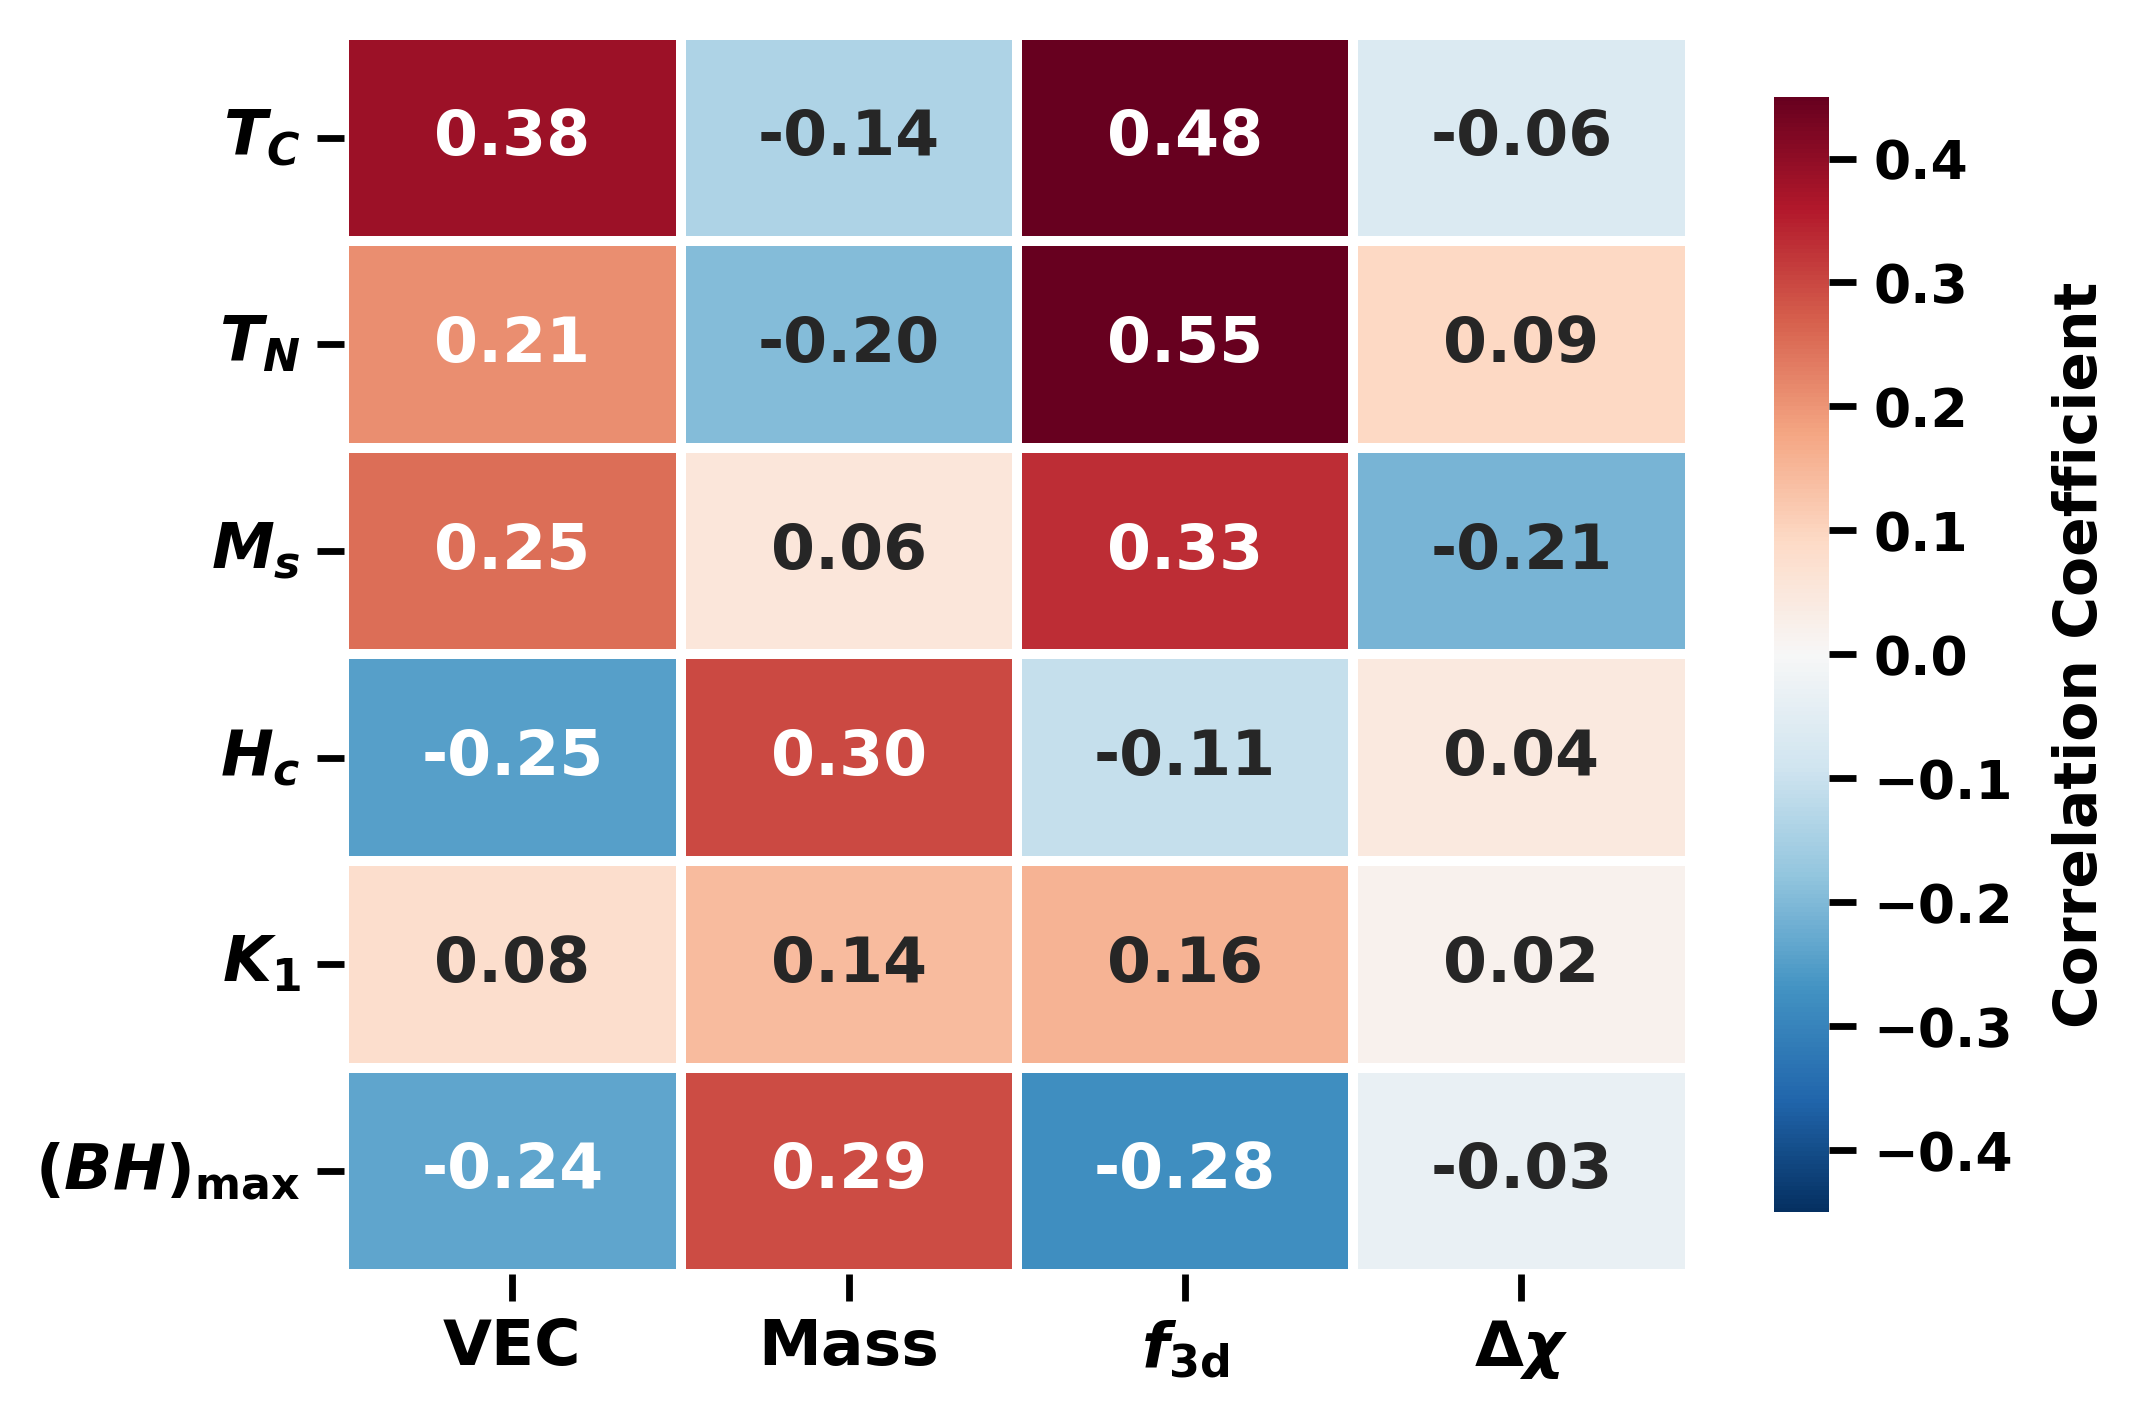
\includegraphics[width=\textwidth]{figures/corr_spearman.png}
    \caption{Spearman Rank Correlation ($\rho$)}
  \end{subfigure}
  \vspace{-0.3em}
  \caption{\textbf{Correlation Structures.} Linear and rank dependencies between compositional descriptors and macroscopic magnetic performance metrics.}
  \label{fig:corrs}
\end{figure}

\begin{itemize}[leftmargin=*]
  \item \textbf{Transition-Metal Fraction ($f_{3d}$):} Strongly drives Curie temperature ($r = 0.45$) and saturation magnetization ($r = 0.31$) through direct $3d\text{--}3d$ quantum exchange.
  \item \textbf{Rare-Earth Concentration ($f_{\text{RE}}$):} Governs magnetocrystalline anisotropy ($K_1$) and coercivity ($H_c$) via localized $4f$ orbital moments and strong spin-orbit coupling.
  \item \textbf{Valence Electron Count ($\text{VEC}$):} Modulates rigid-band filling, exhibiting a negative correlation with energy product ($(BH)_{\max}$, $r = -0.24$) due to trade-offs between high moment and high coercivity.
\end{itemize}

% =========================================================================
\section{Trained Machine Learning \& 3D Foundation AI}
% =========================================================================

The discovery platform integrates trained multi-task models to deliver experimental property estimates alongside physical bounds:

\begin{infobox}{1. Magnetic Phase Classification \& Temperature Routing}
\begin{itemize}[leftmargin=*]
  \item \textbf{Trained Classifier (\texttt{phase\_clf}):} Multi-model ensemble (LightGBM, XGBoost, CatBoost, ExtraTrees, RF) combined with MagFormer compositional transformer embeddings, achieving \textbf{91.9\% Accuracy} and \textbf{0.908 Macro $F_1$}.
  \item \textbf{Dynamic Temperature Routing:}
  \begin{itemize}
    \item If \textbf{Ferromagnetic (FM)}: Evaluates the trained $T_C$ regressor ($R^2 = 0.816$, MAE $= 69.8\text{ K}$) and outputs the Curie point.
    \item If \textbf{Antiferromagnetic (AFM)}: Evaluates the trained $T_N$ regressor ($R^2 = 0.741$, MAE $= 48.6\text{ K}$) and outputs the Néel point, zeroing net moment.
    \item If \textbf{Non-Magnetic (NM)}: Zeroes ordering temperature and net magnetization.
  \end{itemize}
\end{itemize}
\end{infobox}

\begin{infobox}{2. Extrinsic Regressors with Conformal Uncertainty}
\begin{itemize}[leftmargin=*]
  \item \textbf{Trained Ensembles:} Multi-task regressors predict $M_s$, $K_1$, $H_c$, and $(BH)_{\max}$.
  \item \textbf{Non-Parametric Conformal Bounds:} Delivers rigorous 90\% confidence intervals without assuming Gaussian residuals, providing trustworthy margins of uncertainty.
\end{itemize}
\end{infobox}

\begin{infobox}{3. Pretrained 3D Structural Foundation Models}
\begin{itemize}[leftmargin=*]
  \item \textbf{DAO (Diffusion for Atomistic Ordering):} Generates relaxed 3D crystal unit cells directly from stoichiometry and evaluates thermodynamic stability ($E_{\text{hull}} < 0.1\text{ eV/atom}$).
  \item \textbf{MACE (Higher-Order Equivariant Transformer):} Encodes 3D coordination polyhedra and site symmetries, resolving polymorphs sharing the same stoichiometry (e.g., ferromagnetic $\tau$-MnAl vs.\ paramagnetic $\beta$-MnAl).
\end{itemize}
\end{infobox}

% =========================================================================
\section{Inverse Target Discovery \& Pareto Screening}
% =========================================================================

Instead of trial-and-error chemistry, the inverse design engine screens candidates against motor application criteria:
\begin{equation}
(BH)_{\max} \ge 120\text{ kJ/m}^3, \quad T_C \ge 450\text{ K}, \quad \text{Rare-Earth Free}
\end{equation}

\begin{figure}[htbp]
  \centering
  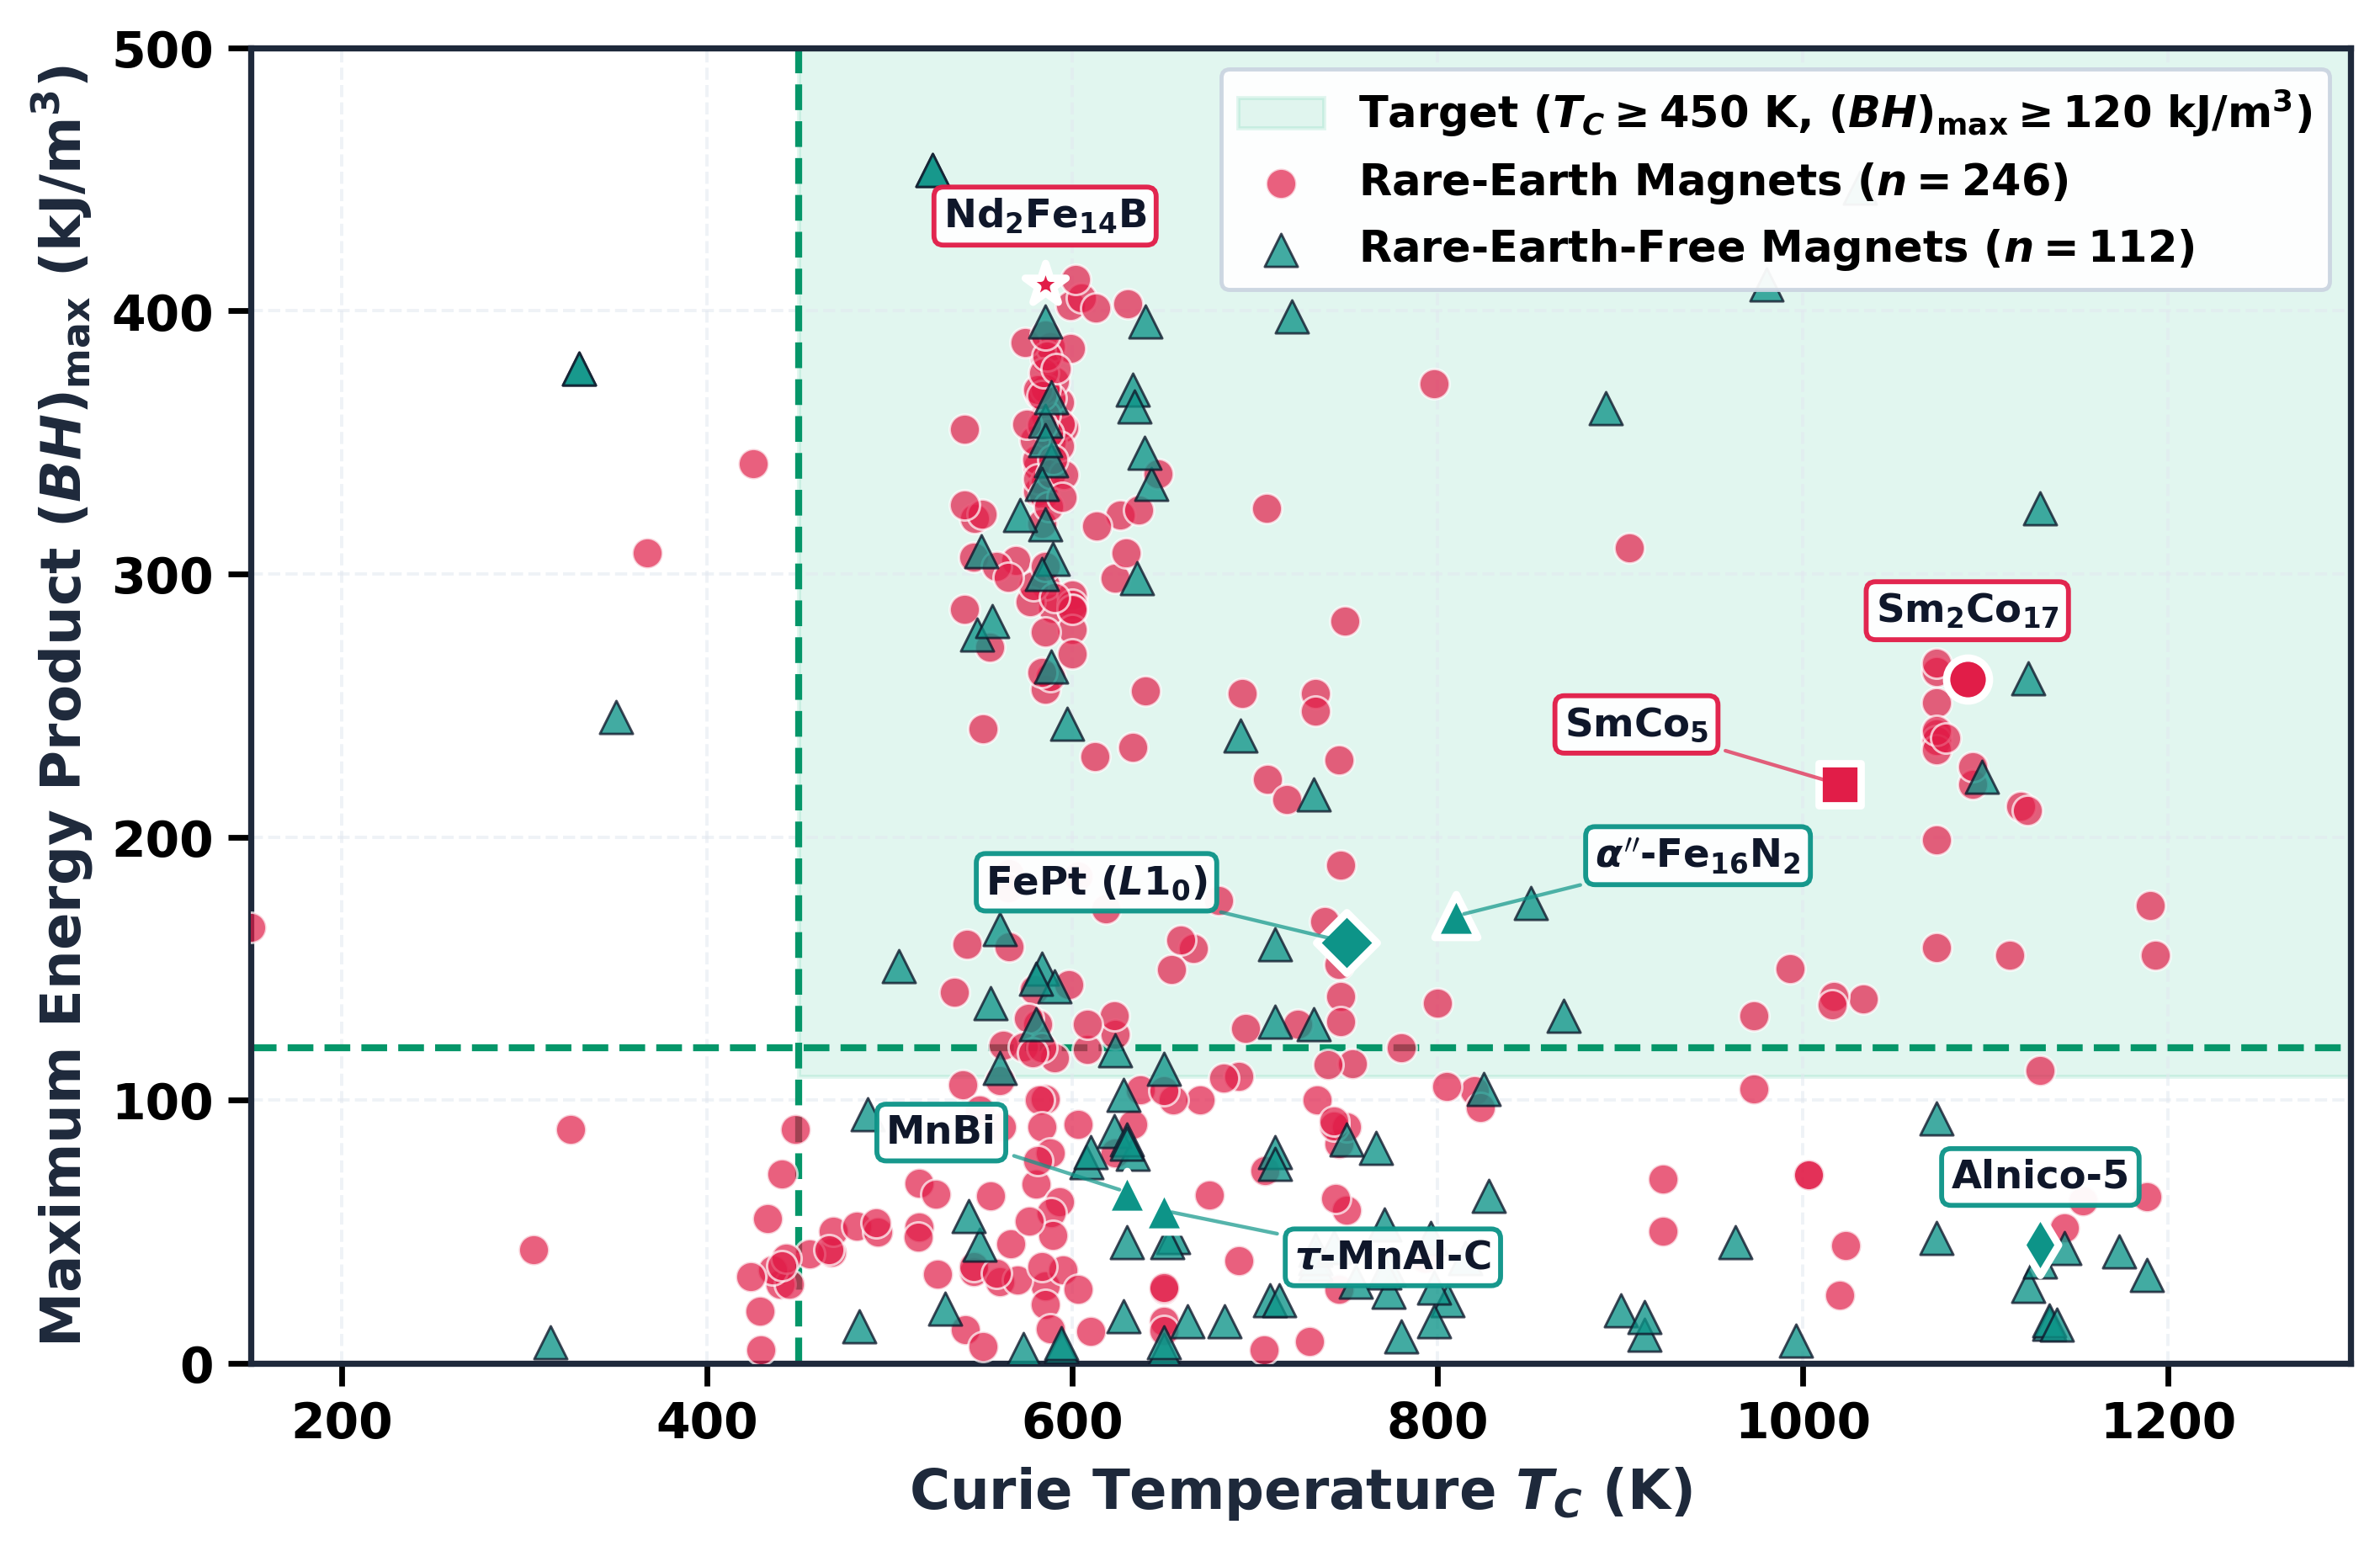
\includegraphics[width=0.82\textwidth]{figures/candidate_pareto.png}
  \vspace{-0.3em}
  \caption{\textbf{Inverse Pareto Frontier.} Energy product $(BH)_{\max}$ vs.\ Curie temperature $T_C$. The green shaded box represents the target zone for rare-earth-free permanent magnets.}
  \label{fig:pareto}
\end{figure}

\textbf{Promising Rare-Earth-Free Candidates on the Pareto Frontier:}
\begin{enumerate}[leftmargin=*]
  \item \textbf{$\text{FeNi (L1}_0\text{ "Tetrataenite")}$:} Predicted $(BH)_{\max} \approx 335\text{ kJ/m}^3$ and $T_C \approx 820\text{ K}$. Highly promising, limited primarily by low-temperature atomic ordering kinetics.
  \item \textbf{$\tau\text{-MnAl}$:} Metastable ferromagnetic phase ($T_C \approx 650\text{ K}, (BH)_{\max} \approx 60\text{--}80\text{ kJ/m}^3$), free of critical elements.
  \item \textbf{$\text{Fe}_{16}\text{N}_2$:} Giant saturation magnetization compound with high theoretical energy product headroom.
\end{enumerate}

% =========================================================================
\section{Interactive Exploration via the Web Platform}
% =========================================================================

The entire workflow is accessible interactively via Streamlit:

\begin{figure}[htbp]
  \centering
  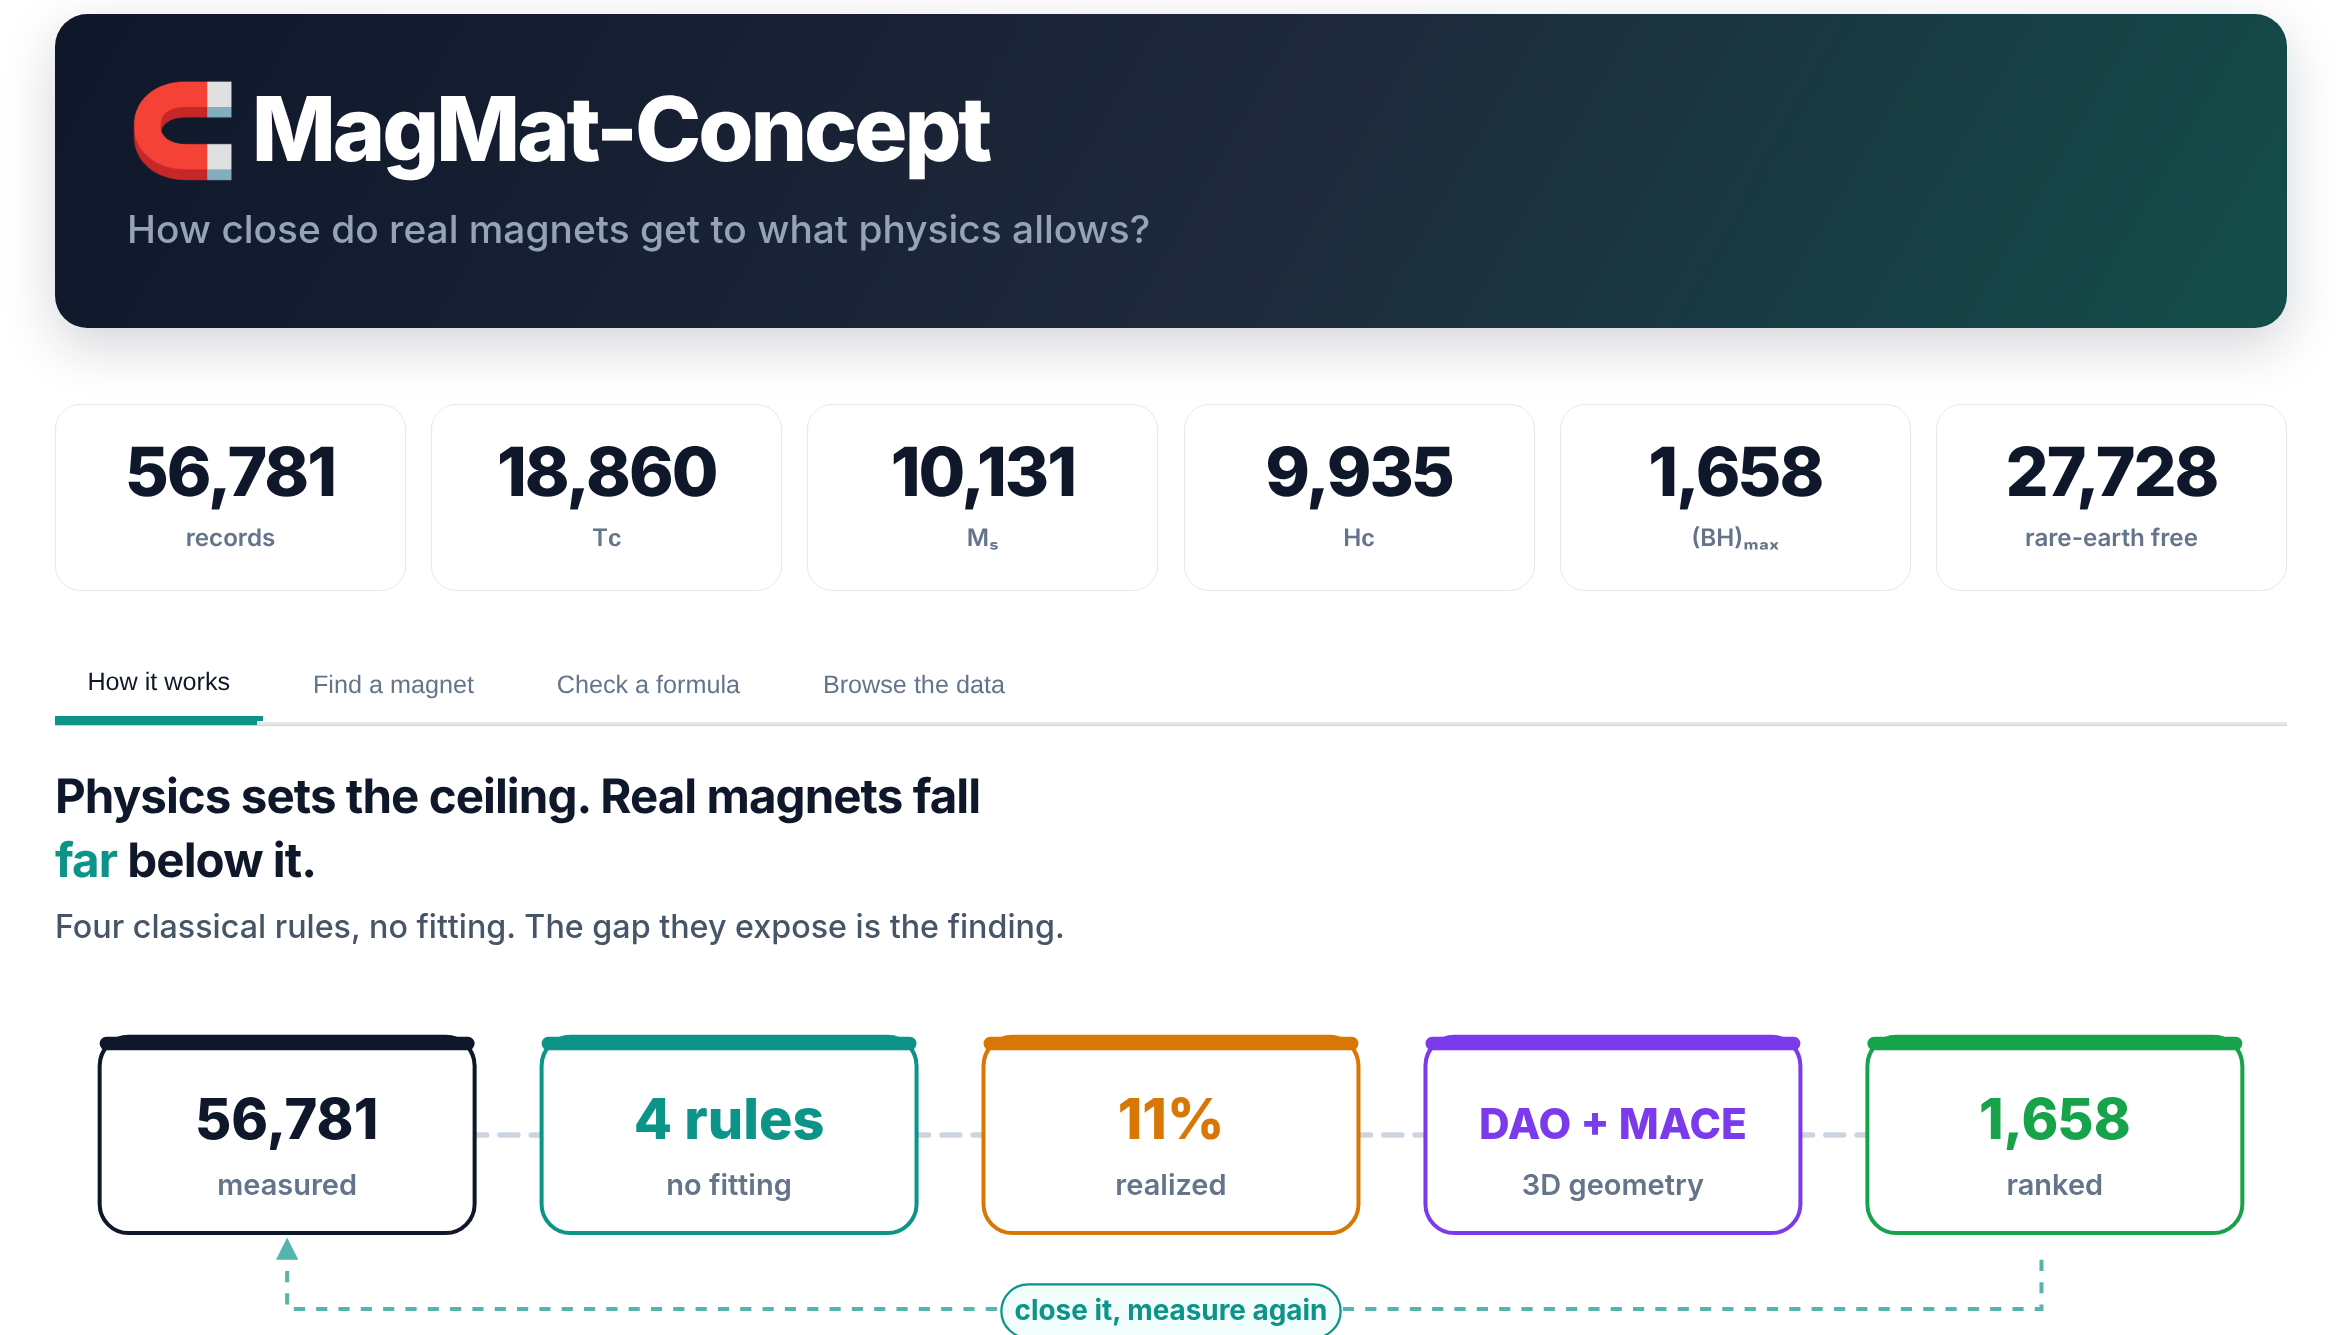
\includegraphics[width=0.88\textwidth]{figures/simple_app_screenshot.png}
  \vspace{-0.3em}
  \caption{\textbf{The Interactive Discovery Platform.} Providing real-time property prediction, 3D unit cell rendering, physical bound calculation, and Pareto candidate exploration.}
  \label{fig:app}
\end{figure}

\begin{center}
\textbf{Launch Command:} \quad \texttt{streamlit run app/app.py}
\end{center}

% =========================================================================
\section{Summary: Physics vs.\ Machine Learning Roles}
% =========================================================================

\begin{table}[htbp]
\centering
\small
\renewcommand{\arraystretch}{1.2}
\begin{tabularx}{\textwidth}{lp{4.2cm}X}
\toprule
\textbf{Framework Layer} & \textbf{What It Provides} & \textbf{Role in Materials Discovery} \\
\midrule
\textbf{Analytical Ceilings} & Slater-Pauling, Stoner, Kronmüller ($H_K$), and Maxwell limits (parameter-free physical laws). & Serves as an unbending theoretical guardrail; discards unphysical proposals and calculates theoretical headroom. \\
\textbf{Trained ML Models} & Predictions for Phase (FM/AFM/NM), $T_C$, $T_N$, $M_s$, $K_1$, $H_c$, and $(BH)_{\max}$ with 90\% conformal bounds. & Predicts realistic experimental performance and polycrystal properties on harmonized datasets. \\
\textbf{3D Foundation AI} & DAO crystal diffusion ($E_{\text{hull}}$) and MACE equivariant symmetry representations. & Supplies the spatial and symmetry descriptors needed to bridge the 89\% microstructural coercivity defect gap. \\
\textbf{Inverse Engine} & Multi-objective Pareto optimization against motor thresholds ($(BH)_{\max} \ge 120\text{ kJ/m}^3, T_C \ge 450\text{ K}$). & Prioritizes high-value, sustainable candidate phases for laboratory synthesis. \\
\bottomrule
\end{tabularx}
\caption{Synergy between physical ceilings, machine learning, and foundation models.}
\label{tab:summary}
\end{table}

\begin{center}
\vspace{0.8em}
\rule{0.5\textwidth}{0.4pt}\\[0.5em]
{\small\sffamily\color{gray} MagMat $\cdot$ Author: Sachin Poudel $\cdot$ September 2026}
\end{center}

\end{document}
